% Options for packages loaded elsewhere
\PassOptionsToPackage{unicode}{hyperref}
\PassOptionsToPackage{hyphens}{url}
\PassOptionsToPackage{dvipsnames,svgnames,x11names}{xcolor}
%
\documentclass[
  12pt,
]{article}

\usepackage{amsmath,amssymb}
\usepackage{setspace}
\usepackage{iftex}
\ifPDFTeX
  \usepackage[T1]{fontenc}
  \usepackage[utf8]{inputenc}
  \usepackage{textcomp} % provide euro and other symbols
\else % if luatex or xetex
  \usepackage{unicode-math}
  \defaultfontfeatures{Scale=MatchLowercase}
  \defaultfontfeatures[\rmfamily]{Ligatures=TeX,Scale=1}
\fi
\usepackage{lmodern}
\ifPDFTeX\else  
    % xetex/luatex font selection
\fi
% Use upquote if available, for straight quotes in verbatim environments
\IfFileExists{upquote.sty}{\usepackage{upquote}}{}
\IfFileExists{microtype.sty}{% use microtype if available
  \usepackage[]{microtype}
  \UseMicrotypeSet[protrusion]{basicmath} % disable protrusion for tt fonts
}{}
\makeatletter
\@ifundefined{KOMAClassName}{% if non-KOMA class
  \IfFileExists{parskip.sty}{%
    \usepackage{parskip}
  }{% else
    \setlength{\parindent}{0pt}
    \setlength{\parskip}{6pt plus 2pt minus 1pt}}
}{% if KOMA class
  \KOMAoptions{parskip=half}}
\makeatother
\usepackage{xcolor}
\setlength{\emergencystretch}{3em} % prevent overfull lines
\setcounter{secnumdepth}{5}
% Make \paragraph and \subparagraph free-standing
\ifx\paragraph\undefined\else
  \let\oldparagraph\paragraph
  \renewcommand{\paragraph}[1]{\oldparagraph{#1}\mbox{}}
\fi
\ifx\subparagraph\undefined\else
  \let\oldsubparagraph\subparagraph
  \renewcommand{\subparagraph}[1]{\oldsubparagraph{#1}\mbox{}}
\fi
\pagestyle{empty}


\providecommand{\tightlist}{%
  \setlength{\itemsep}{0pt}\setlength{\parskip}{0pt}}\usepackage{longtable,booktabs,array}
\usepackage{calc} % for calculating minipage widths
% Correct order of tables after \paragraph or \subparagraph
\usepackage{etoolbox}
\makeatletter
\patchcmd\longtable{\par}{\if@noskipsec\mbox{}\fi\par}{}{}
\makeatother
% Allow footnotes in longtable head/foot
\IfFileExists{footnotehyper.sty}{\usepackage{footnotehyper}}{\usepackage{footnote}}
\makesavenoteenv{longtable}
\usepackage{graphicx}
\makeatletter
\def\maxwidth{\ifdim\Gin@nat@width>\linewidth\linewidth\else\Gin@nat@width\fi}
\def\maxheight{\ifdim\Gin@nat@height>\textheight\textheight\else\Gin@nat@height\fi}
\makeatother
% Scale images if necessary, so that they will not overflow the page
% margins by default, and it is still possible to overwrite the defaults
% using explicit options in \includegraphics[width, height, ...]{}
\setkeys{Gin}{width=\maxwidth,height=\maxheight,keepaspectratio}
% Set default figure placement to htbp
\makeatletter
\def\fps@figure{htbp}
\makeatother
\newlength{\cslhangindent}
\setlength{\cslhangindent}{1.5em}
\newlength{\csllabelwidth}
\setlength{\csllabelwidth}{3em}
\newlength{\cslentryspacingunit} % times entry-spacing
\setlength{\cslentryspacingunit}{\parskip}
\newenvironment{CSLReferences}[2] % #1 hanging-ident, #2 entry spacing
 {% don't indent paragraphs
  \setlength{\parindent}{0pt}
  % turn on hanging indent if param 1 is 1
  \ifodd #1
  \let\oldpar\par
  \def\par{\hangindent=\cslhangindent\oldpar}
  \fi
  % set entry spacing
  \setlength{\parskip}{#2\cslentryspacingunit}
 }%
 {}
\usepackage{calc}
\newcommand{\CSLBlock}[1]{#1\hfill\break}
\newcommand{\CSLLeftMargin}[1]{\parbox[t]{\csllabelwidth}{#1}}
\newcommand{\CSLRightInline}[1]{\parbox[t]{\linewidth - \csllabelwidth}{#1}\break}
\newcommand{\CSLIndent}[1]{\hspace{\cslhangindent}#1}

\usepackage{geometry}
\geometry{paper=a4paper,margin=1in}
\usepackage{fontspec}
\setmainfont{Arial}
\setlength{\tabcolsep}{2pt}
\setlength{\parskip}{12pt}
\usepackage{float}
\floatplacement{figure}{H}
\makeatletter
\makeatother
\makeatletter
\makeatother
\makeatletter
\@ifpackageloaded{caption}{}{\usepackage{caption}}
\AtBeginDocument{%
\ifdefined\contentsname
  \renewcommand*\contentsname{Table of contents}
\else
  \newcommand\contentsname{Table of contents}
\fi
\ifdefined\listfigurename
  \renewcommand*\listfigurename{List of Figures}
\else
  \newcommand\listfigurename{List of Figures}
\fi
\ifdefined\listtablename
  \renewcommand*\listtablename{List of Tables}
\else
  \newcommand\listtablename{List of Tables}
\fi
\ifdefined\figurename
  \renewcommand*\figurename{Figure}
\else
  \newcommand\figurename{Figure}
\fi
\ifdefined\tablename
  \renewcommand*\tablename{Table}
\else
  \newcommand\tablename{Table}
\fi
}
\@ifpackageloaded{float}{}{\usepackage{float}}
\floatstyle{ruled}
\@ifundefined{c@chapter}{\newfloat{codelisting}{h}{lop}}{\newfloat{codelisting}{h}{lop}[chapter]}
\floatname{codelisting}{Listing}
\newcommand*\listoflistings{\listof{codelisting}{List of Listings}}
\makeatother
\makeatletter
\@ifpackageloaded{caption}{}{\usepackage{caption}}
\@ifpackageloaded{subcaption}{}{\usepackage{subcaption}}
\makeatother
\makeatletter
\@ifpackageloaded{tcolorbox}{}{\usepackage[skins,breakable]{tcolorbox}}
\makeatother
\makeatletter
\@ifundefined{shadecolor}{\definecolor{shadecolor}{rgb}{.97, .97, .97}}
\makeatother
\makeatletter
\makeatother
\makeatletter
\makeatother
\ifLuaTeX
  \usepackage{selnolig}  % disable illegal ligatures
\fi
\IfFileExists{bookmark.sty}{\usepackage{bookmark}}{\usepackage{hyperref}}
\IfFileExists{xurl.sty}{\usepackage{xurl}}{} % add URL line breaks if available
\urlstyle{same} % disable monospaced font for URLs
\hypersetup{
  pdftitle={Mapping India in Pliny the Elder's Natural History},
  pdfauthor={Dawn, Lizao Zhuang (r0914937)},
  pdfkeywords={Natural History, Pliny the Elder, Spatial
Humanities, Indo-Roman, Indo-Mediterranean},
  colorlinks=true,
  linkcolor={blue},
  filecolor={Maroon},
  citecolor={Blue},
  urlcolor={Blue},
  pdfcreator={LaTeX via pandoc}}

\title{Mapping India in Pliny the Elder's \emph{Natural History}}
\author{Dawn, Lizao Zhuang (r0914937)}
\date{}

\begin{document}
\maketitle
\begin{abstract}
this is an abstract
\end{abstract}
\ifdefined\Shaded\renewenvironment{Shaded}{\begin{tcolorbox}[frame hidden, enhanced, borderline west={3pt}{0pt}{shadecolor}, interior hidden, boxrule=0pt, sharp corners, breakable]}{\end{tcolorbox}}\fi

\renewcommand*\contentsname{Table of Contents}
{
\hypersetup{linkcolor=}
\setcounter{tocdepth}{3}
\tableofcontents
}
\listoffigures
\listoftables
\setstretch{1.15}
\clearpage
\pagestyle{plain}
\pagenumbering{arabic}  
\setcounter{page}{1}

\hypertarget{sec-introduction}{%
\section{Introduction}\label{sec-introduction}}

\hypertarget{natural-history-and-its-complexity}{%
\subsection{\texorpdfstring{\emph{Natural History} and its
complexity}{Natural History and its complexity}}\label{natural-history-and-its-complexity}}

Pliny the Elder's \emph{Natural History} is widely recognized as the
earliest encyclopedia in the world, manifesting a pioneering effort in
comprehensively cataloging the vast array of human knowledge from that
era.

The work is thematically divided into 37 books, covering a diverse range
of subjects including astronomy, geography, zoology, botany, medicine,
and more. Pliny meticulously consulted a wide range of Greek and Roman
references, totaling approximately 2,000 volumes\footnote{\emph{Natural
  History} 1.5.1 (https://topostext.org/work/148)}, and interwove his
own literary interpretation or comments to the narratives.

Despite the carefully designed knowledge-ordering framework (Lao 2016),
scholars have observed a paradoxical complexity in \emph{Natural
History}, evident in its linguistic style, narrative approach, and use
of references. The work compiles inconsistent toponyms from Greek and
Latin, includes digressions in descriptions (Roller 2022), and exhibits
changes in vocabularies and sentence structures (Pinkster 2005).
However, it is precisely this complexity that makes the work more
fascinating and not only a valuable source of the knowledge and
worldview of the ancient world, but also a gateway into Pliny's
conceptualization, imagination, and even the prevailing imperial
ideology of that time.

The complexity and interconnectivity of the general structure of
\emph{Natural History} are further highlighted in different aspects by
refreshing approaches. For the content organisation, Healy (1999)
advocated Pliny's original contribution in revealing the technology and
science engagement of the Rome Empire. Taking the historical, political
and linguistic context into consideration, he found that in addition to
providing informative descriptions of natural phenomena and scientific
experiments, Pliny also developed the scientific language in Latin
through his work. And Naas (2002) discussed how Pliny formulated the
diverse materials into his encyclopaedic structure, revealing the work's
multifaceted nature as an epistemological, ideological, and moral
project. Analysing Pliny's employment of the historical exemplum in the
work, Schultze (2011) argued how that literary device directed and
teased the readers as well as established a profound connection between
human beings and the entire spectrum of nature in \emph{Natural
History}.

In addition to the close reading methods used in the above analyses of
the context and references in \emph{Natural History}, Rydberg-Cox (2021)
employed network analysis method with different metrics to map the
interrelationships between Pliny's sources and the topics discussed in
the work. Furthermore, Fantoli (2022) presented a comparative study of
book 2 of \emph{Natural History} and book 7 of Seneca's work
\emph{Natural Questions}, both of which are astronomy sections in the
Latin classics about nature. Her study utilized statistical method to
analyse variations in their discourse distribution, and identified
Pliny's unique stylistic features. The encyclopaedic authorial intent
shown in \emph{Natural History} is also vindicated through
correspondence and tree analysis. These two studies demonstrate how
distant reading methodologies offer novel insights into our
understanding of the ancient treatises.

In addition to the contextual and referential analyses about
\emph{Natural History}, Rydberg-Cox (2021) employed network analysis
techniques, applying various metrics to illustrate the connections
between Pliny's sources and the topics discussed in the work.
Furthermore, Fantoli (2022) conducted a comparative examination of book
2 of \emph{Natural History} and book 7 of Seneca's \emph{Natural
Questions}, both focused on astronomy as part of the Latin classics
about nature. Statistical methods were applied to investigate variations
in their discursive distribution, effectively identifying Pliny's
distinctive stylistic attributes. Moreover, the encyclopaedic authorial
intent evident in \emph{Natural History} is validated through
correspondence and tree analysis. These studies collectively showcase
how distant reading methodologies offer novel insights into our
understanding of ancient treatises.

\hypertarget{spatial-perstpective-in-natural-history}{%
\subsection{\texorpdfstring{Spatial perstpective in \emph{Natural
History}}{Spatial perstpective in Natural History}}\label{spatial-perstpective-in-natural-history}}

As pointed out by Beagon (2011), differentiating from his predecessors,
Pliny showed a ``terrestrial curiosity'' in \emph{Natural History},
emphasising recognition of the physical, material world. In this regard,
the vision of geography plays a pivotal role in distributing
information, knowledge, and events throughout \emph{Natural History}.

Drawing from the long-established topographical and ethnographic
traditions, Pliny seamlessly connects volumes dedicated to geography
(books 3-6) with broader elements, activities, and cultural, historical,
and societal contexts(Roller 2022), exemplified in his portrayal of
exotic plants, communities' habitats, imperial expeditions, and trade
products. In other words, geographical names that occurred in each book
of \emph{Natural History} served as signposts guiding readers through
diverse lands, shedding light on how Pliny and his contemporaries
perceived and conceptualized the world around them.

A normalized frequency of place name occurrence in the work is
calculated as the ratio of counts of the occurrences of place names in
each book to the word lengths of the book
(Table~\ref{tbl-place_book_distribution}). The bar chart
(Figure~\ref{fig-place_distribution}) depicts the comparison of the
distribution of place names in the books of \emph{Natural History}. The
observation aligns with the content structure of \emph{Natural History},
that books 3-6 centred around the themes of ``geography and
ethnography'', contain the most mentions of location names, and place
names are also frequently mentioned in books about agriculture and
horticulture (book 12-14), aquatic life (book 31), and mining and
mineralogy (book 34-37).

\hypertarget{tbl-place_book_distribution}{}
\begin{longtable}[]{@{}llll@{}}
\caption{\label{tbl-place_book_distribution}Normalized distribution of
place names in \emph{Natural History}}\tabularnewline
\toprule\noalign{}
& Total\_length & Place\_count & Place\_freq \\
Book & & & \\
\midrule\noalign{}
\endfirsthead
\toprule\noalign{}
& Total\_length & Place\_count & Place\_freq \\
Book & & & \\
\midrule\noalign{}
\endhead
\bottomrule\noalign{}
\endlastfoot
1 & 2778 & 1 & 0.000360 \\
2 & 30570 & 406 & 0.013281 \\
3 & 18037 & 1007 & 0.055830 \\
4 & 15434 & 1309 & 0.084813 \\
5 & 18872 & 1112 & 0.058923 \\
6 & 27891 & 1012 & 0.036284 \\
7 & 21204 & 225 & 0.010611 \\
8 & 24176 & 185 & 0.007652 \\
9 & 19197 & 140 & 0.007293 \\
10 & 20816 & 121 & 0.005813 \\
11 & 27345 & 77 & 0.002816 \\
12 & 13906 & 188 & 0.013519 \\
13 & 13243 & 164 & 0.012384 \\
14 & 15277 & 189 & 0.012372 \\
15 & 14552 & 135 & 0.009277 \\
16 & 25442 & 180 & 0.007075 \\
17 & 29387 & 82 & 0.002790 \\
18 & 35850 & 222 & 0.006192 \\
19 & 18822 & 146 & 0.007757 \\
20 & 22743 & 21 & 0.000923 \\
21 & 17896 & 95 & 0.005308 \\
22 & 16491 & 24 & 0.001455 \\
23 & 15764 & 17 & 0.001078 \\
24 & 17491 & 56 & 0.003202 \\
25 & 16734 & 85 & 0.005079 \\
26 & 15448 & 35 & 0.002266 \\
27 & 12444 & 40 & 0.003214 \\
28 & 26476 & 28 & 0.001058 \\
29 & 13976 & 31 & 0.002218 \\
30 & 14395 & 23 & 0.001598 \\
31 & 12204 & 222 & 0.018191 \\
32 & 14635 & 76 & 0.005193 \\
33 & 17946 & 113 & 0.006297 \\
34 & 18972 & 193 & 0.010173 \\
35 & 21283 & 277 & 0.013015 \\
36 & 21295 & 357 & 0.016764 \\
37 & 22255 & 282 & 0.012671 \\
\end{longtable}

\begin{figure}

{\centering 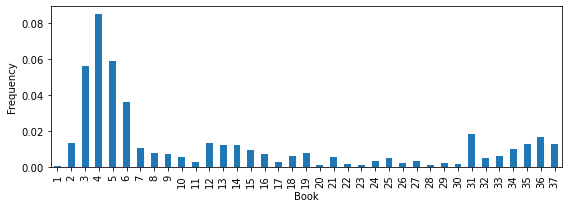
\includegraphics{NHthesis_structure_files/figure-pdf/fig-place_distribution-output-1.png}

}

\caption{\label{fig-place_distribution}Normalized distribution of place
names in \emph{Natural History}}

\end{figure}

\hypertarget{text-source-for-the-study}{%
\subsection{Text source for the study}\label{text-source-for-the-study}}

\emph{Natural History} is originally in Latin. For the purpose of this
study, an English translation conducted by Henry T. Riley (1816-1878)
and John Bostock (1773-1846), first published in 1855, is utilized. The
translated text is obtained in a digitized version from the
\href{https://topostext.org/the-project}{TOPOSText project}, having been
sourced from the Perseus Project and governed by a Creative Commons
Attribution-Share-Alike 3.0 U.S. License.

Annotations of proper names, place names and their corresponding
coordinates are available together with the text of \emph{Natural
History} (\href{https://topostext.org/work/148}{Book1-11},
\href{https://topostext.org/work/153}{Book12-37}) on
\href{https://topostext.org/the-project}{TOPOSText project}. This
invaluable resource allows for creating a dataset that includes both the
textual contents and geographical annotations, which can be utilized to
investigate the distribution of place names in the entire work and
examine the frequencies and patterns of geography-related content.

The extension of the extracted corpora and the workflow of the
extraction will be further explained in the Methodology chapter
(Section~\ref{sec-methodology}).

\hypertarget{sec-research_question}{%
\section{Research Question}\label{sec-research_question}}

\hypertarget{prominent-mentioned-places-in-natural-history}{%
\subsection{\texorpdfstring{Prominent mentioned places in \emph{Natural
History}}{Prominent mentioned places in Natural History}}\label{prominent-mentioned-places-in-natural-history}}

Based on the geographical annotations in \emph{Natural History} provided
by the TOPOSText, there are 2052 unique places mentioned in
\emph{Natural History}.

The top 20 most frequently mentioned place names (as 1\% of the total)
in \emph{Natural History} is shown in Table~\ref{tbl-topplace}.

\hypertarget{tbl-topplace}{}
\begin{longtable}[]{@{}llllll@{}}
\caption{\label{tbl-topplace}Top 20 mentioned place names in Natural
History}\tabularnewline
\toprule\noalign{}
& ToposText\_ID & Place\_Name & Lat & Long & Count \\
\midrule\noalign{}
\endfirsthead
\toprule\noalign{}
& ToposText\_ID & Place\_Name & Lat & Long & Count \\
\midrule\noalign{}
\endhead
\bottomrule\noalign{}
\endlastfoot
1687 & https://topostext.org/place/406163RIta & Italy & 40.6000 &
16.30000 & 292 \\
2034 & https://topostext.org/place/419125PRom & Rome & 41.8910 &
12.48600 & 269 \\
52 & https://topostext.org/place/271307REgy & Egypt & 27.1000 & 30.70000
& 261 \\
82 & https://topostext.org/place/300740RInd & India & 30.0000 & 74.00000
& 167 \\
57 & https://topostext.org/place/280400RAra & Arabia & 28.0000 &
40.00000 & 123 \\
320 & https://topostext.org/place/355390RSyr & Syria & 35.5000 &
39.00000 & 109 \\
255 & https://topostext.org/place/350330RCyp & Cyprus & 35.0000 &
33.00000 & 85 \\
109 & https://topostext.org/place/312301WNil & Nile & 30.0918 & 31.23130
& 85 \\
2282 & https://topostext.org/place/441073LAlp & Alps & 44.1420 & 7.34300
& 82 \\
766 & https://topostext.org/place/376145RSic & Sicily & 37.6000 &
14.50000 & 71 \\
275 & https://topostext.org/place/352252IKre & Crete & 35.2052 &
25.18360 & 64 \\
7 & https://topostext.org/place/130350REth & Ethiopia & 13.0100 &
35.01000 & 58 \\
417 & https://topostext.org/place/364282IRho & Rhodes & 36.4408 &
28.22440 & 56 \\
966 & https://topostext.org/place/380237PAth & Athens & 37.9718 &
23.72793 & 56 \\
2043 & https://topostext.org/place/419125SCap & Capitol & 41.8933 &
12.48300 & 52 \\
298 & https://topostext.org/place/353403WEup & Euphrates & 35.2791 &
40.27080 & 47 \\
2241 & https://topostext.org/place/435335WPon & Pontus & 43.5000 &
33.50000 & 47 \\
1839 & https://topostext.org/place/411146RCam & Campania & 41.1000 &
14.60000 & 46 \\
1480 & https://topostext.org/place/397443RArm & Armenia & 39.7020 &
44.29800 & 45 \\
17 & https://topostext.org/place/195390WEry & Red Sea & 19.5000 &
39.00000 & 42 \\
545 & https://topostext.org/place/369103PCar & Carthage & 36.8500 &
10.32000 & 42 \\
602 & https://topostext.org/place/370340RCil & Cilicia & 37.0100 &
34.01000 & 42 \\
\end{longtable}

The place names referenced in \emph{Natural History} are geographically
mapped, with each location marked on the map using its corresponding
coordinates. A dot is assigned to represent a place, with the size and
color of the dot reflecting the frequency of its mention in the work.
The larger and darker the dot, the more frequently the place is referred
to within the context of \emph{Natural History}.

An intriguing observation from the output, as depicted in
Figure~\ref{fig-geonamemap_pdf}, is the prominence of India, a region
outside the Mediterranean, despite its high frequency of mentions.

\begin{figure}

{\centering 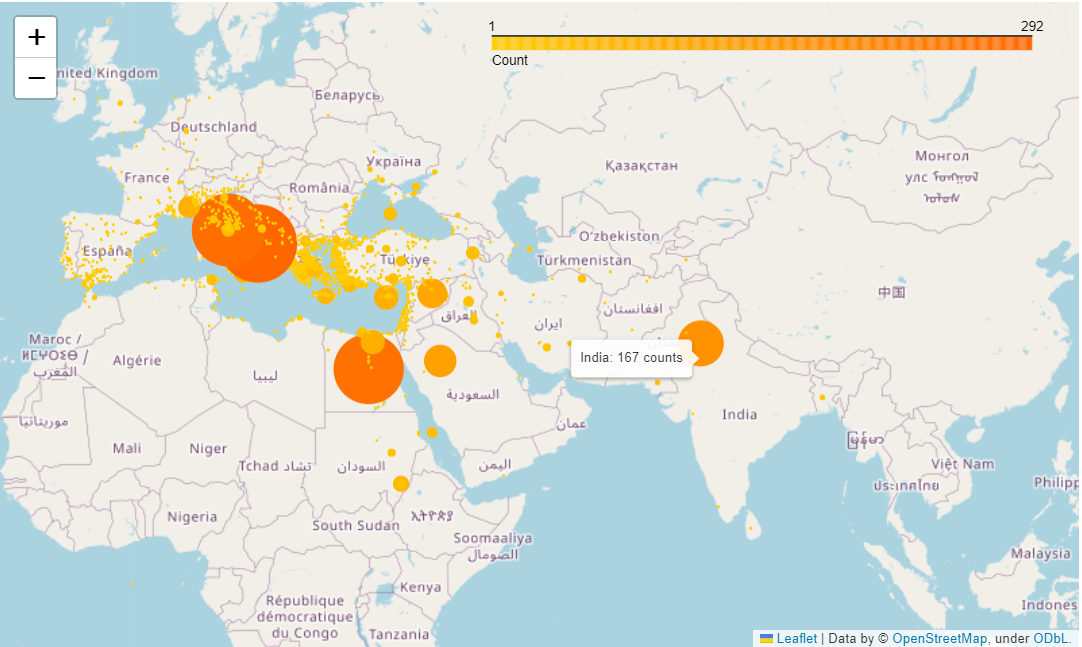
\includegraphics{NHthesis_structure_files/figure-pdf/fig-geonamemap_pdf-output-1.png}

}

\caption{\label{fig-geonamemap_pdf}Place name distribution map}

\end{figure}

\hypertarget{why-india}{%
\subsection{Why India?}\label{why-india}}

Geographically, India seems a distant and disconnected territory from
the Roman Empire, lacking any direct aquatic or land routes with the
Mediterranean region. However, the exotic curiosity Pliny attempted to
integrate within his work, and the history of the Indo-roman trade
relations, can be regarded as a broader context for the prominent
mentioning of India in \emph{Natural History}.

As suggested by (Murphy 2003), the \emph{mirabilia}, encompassing
accounts of extraordinary landscapes, people, plants, and animals,
assumes a substantial proportion within the books of \emph{Natural
History}. Pliny's inclusion of such exotic elements not only catered to
the prevailing curiosity of his Roman readers but also fostered a
comparative perspective between distant locales, exemplified by his
references to India, and their natural counterparts within Rome (Naas
2011). Within a research framework of Roman Imperialism, the detailed
portrayal of foreign lands, such as India, holds significant importance
in shaping both Pliny's and his contemporary Roman readers' perception
of their place within the global landscape (Pollard 2009).

In addition, \emph{Natural History} serves as a valuable reference for
tracking the Indo-Mediterranean network of exchange (Pollard 2009).
Through the depiction of cities, ports, and rivers along the trade
routes, the work provides substantive evidence of the flourishing trade
relations between the Roman Empire and the Indian subcontinent (Neelis
2011). The extensive exemplification of diverse commodities, such as
gemstones, glass, spices, textiles, plants, and wine, along with the
accounts of the currency \emph{sestertii} involved in the merchandise
exchange in the work shed lights to the compelling details and social
and cultural implications of this long-distance trade (Székely 2006;
Pollard 2009). Furthermore, the direct criticisms regarding the high
cost of the luxury items imported from India imply both the magnitude of
the trade volume and Pliny's stance towards this commercial interaction
(Neelis 2011).

\hypertarget{india-related-text-as-a-case-study}{%
\subsection{India-related text as a case
study}\label{india-related-text-as-a-case-study}}

In light of the observations and foundational research mentioned above,
the present study centres its investigation on the spatial perspective
within Pliny's \emph{Natural History}, focusing on the texts about
India, seeking to delve into the discourse surrounding this region. To
achieve this goal, distant reading methodologies, including statistical
analysis, topic modelling, and social network analysis, are employed in
the study.

The main aim of this study is to explore how India is described, and how
the information about India is structured in \emph{Natural History},
which may also contribute to a more profound comprehension of the
inherent complexity and interconnectivity that permeates this monumental
work.

\hypertarget{sec-methodology}{%
\section{Methodology}\label{sec-methodology}}

\hypertarget{workflow}{%
\subsection{Workflow}\label{workflow}}

The workflow for this study involves the following key stages:

\textbf{Data Collection}:

As mentioned in the Introduction chapter
(Section~\ref{sec-introduction}), the text employed for this study is
obtained from the digitized English translation (by Henry T. Riley
(1816-1878) and John Bostock (1773-1846)) of Pliny's \emph{Natural
History} available on \href{https://topostext.org/the-project}{TOPOSText
project}.

The two parts of \emph{Natural History}
(\href{https://topostext.org/work/148}{Book1-11},
\href{https://topostext.org/work/153}{Book12-37}) are scraped for their
the textual contents together with the geographical annotation of the
mentioned ancient places, and their book, chapter and paragraph
affiliations with the function provided in
\href{https://www.crummy.com/software/BeautifulSoup/bs4/doc/}{Beautiful
Soup} library of Python.

\textbf{Data Preprocessing}:

The information extracted from the HTML is structured into separate
columns as \href{https://pandas.pydata.org/}{Pandas} dataframe, a
dataframe for plain text of the entire work, and a dataframe for
geographical-related text in \emph{Natural History} with the
geographical annotations are generated and stored in CSV format.

After a preliminary exploration, the research focus is narrowed down to
India-related text in \emph{Natural History}. Referring to the
geographical territories in the scope of ancient Greek and Roman world
(Talbert 2000b), a dataframe for India-related text is filtered from the
abovementioned dataframe for geographical-related text with the range of
corresponding coordinates of Indian subcontinent in the era of
\emph{Natural History}. The flitered India-related text dataframe is
also stored in CSV format.

The location names mentioned in the India-related text were checked
manually for its completeness. The identified location names without
annotation in TOPOSText were appended to the India-related text dataset.

Additionally, the textual contents in the datasets were preprocessed
with tokenization, lemmatization and the exclusion of stop-words
processes.

\textbf{Data Analysis}:

Statistical analysis is conducted in the preliminary exploration of the
extracted dataframes. A nomalized frequency of geographical name
occurence in each book is calculated for an overview of the place name
distribution in \emph{Natural History}. And the top 1\% prominently
mentioned place names in the entire work are sorted out with the time of
their occurencies. The specific attention on India-related text as a
case study is drown from this initial observation.

In the analysis of the India-related text (target corpus) in
\emph{Natural History}, three analysis methods are employed:

\begin{enumerate}
\def\labelenumi{\arabic{enumi}.}
\item
  Word frequency and collocation analysis: single word frequency and
  bi-gram collocation of the target corpus are measured with the
  functions in \href{https://www.nltk.org/}{NLTK} package for an
  overview of the common word patterns relating to India in
  \emph{Natural History}.
\item
  Topic modelling: \href{https://radimrehurek.com/gensim/}{Genism}
  library is used for semantic vectorization and implemetion of Latent
  Dirichlet Allocation (LDA) model for the topic modelling of the target
  corpus, and the library of
  \href{https://pyldavis.readthedocs.io/en/latest/index.htmlgenism}{pyLDAvis}
  is utilized for an interactive visualisation. The output of this
  method shows the potential topics in the India-related text in
  \emph{Natural History}.
\item
  Network analysis for named entities: Person names mentioned in the
  India-related text are retrieved from annotaions on TOPOSText. Person
  and place names occured in the target corpus are extracted as nodes
  together with their affiliated book numbers, and the co-occurence
  between the nodes are counted as edges for network analysis. The
  output of this method is a graph showing the clusters of the nodes in
  the target corpus, indicating the structure of the content related to
  India in \emph{Natural History}.
\end{enumerate}

\textbf{Interpretation and Conclusion}:

The workflow and parameter setting of each research method are explained
at the beginning of each analysis section. The results aquired from each
method are interpreted with a dialouge to the broader literature and
close reading of the related text.

In the Conclusion chapter (Section~\ref{sec-conclusions}), the findings
are illustrated comprehensively as a response to the research questions.
And the limitations of the methods are discussed and evaluated.

\hypertarget{data-preparation}{%
\subsection{Data preparation}\label{data-preparation}}

This section provides an overview of the data preparation process,
encompassing four sub-sections: HTML scraping from TOPOSText, creation
of a filtered dataset of ``India-related text,'' completeness check and
preprocessing of textual data. The tools and procedures employed in data
collection and dataset generation for the study are introduced in the
subsequent content.

\hypertarget{html-scraping-from-topostext}{%
\subsubsection{HTML scraping from
TOPOSText}\label{html-scraping-from-topostext}}

As previously stated, the textual contents of Pliny's \emph{Natural
History} are available on the
\href{https://topostext.org/the-project}{TOPOSText project}, presented
in two distinct parts: \href{https://topostext.org/work/148}{Book 1-11},
\href{https://topostext.org/work/153}{Book 12-37}. Both parts are
provided in HTML format, offering separate sections of the complete
work.

To extract the relevant data, the
\href{https://www.crummy.com/software/BeautifulSoup/bs4/doc/}{Beautiful
Soup} tool, a Python library renowned for parsing HTML and XML
documents, was employed.

The text in the HTML documents is organised into paragraphs, each
uniquely identified by an ``id'' attribute that specifies its
corresponding book, chapter, and paragraph number. For instance, a
typical paragraph has an ``id'' tag as follows:

\textbf{\textless p
id=`urn:cts:latinLit:phi0978.phi001:3.9.7'\textgreater{}}

The textual contents are retrieved with the information from these
``id'' attributes and structured as a reference dataset, comprising the
plain text of \emph{Natural History} divided into paragraphs, with each
paragraph assigned a unique identifier, and separate columns indicating
its affiliated book, chapter, and paragraph number. An illustrative
example of the dataset's structure is shown as
Table~\ref{tbl-dataset_plaintext}.

\hypertarget{tbl-dataset_plaintext}{}
\begin{longtable}[]{@{}lllllll@{}}
\caption{\label{tbl-dataset_plaintext}Example for the reference dataset
containing the plain text in paragraphs of \emph{Natural
History}}\tabularnewline
\toprule\noalign{}
& UUID4 & Reference & Book & Chapter & Paragraph & Text \\
\midrule\noalign{}
\endfirsthead
\toprule\noalign{}
& UUID4 & Reference & Book & Chapter & Paragraph & Text \\
\midrule\noalign{}
\endhead
\bottomrule\noalign{}
\endlastfoot
0 & e9e67565-bb... & urn:cts:lat... & 1 & 1 & 1.0 & PREFACE IN ... \\
1 & 010b853d-b8... & urn:cts:lat... & 1 & 2 & 1.0 & But who cou... \\
2 & 2d10e332-9c... & urn:cts:lat... & 1 & 3 & 1.0 & But if Luci... \\
3 & 113e0b4c-5b... & urn:cts:lat... & 1 & 4 & 1.0 & My own pres... \\
4 & 19115032-9f... & urn:cts:lat... & 1 & 5 & 1.0 & For my own ... \\
\end{longtable}

There are a total of 3493 paragraphs in the English-translated version
of \emph{Natural History} used in this study. The extracted text
contains 343096 tokens and 28606 types after preprocessing. This
reference dataset has been saved in CSV format for record.

Moreover, the geographical annotations concerning the ancient places
mentioned in the text are labelled with a class attribute denoted as
``place'', including a URI for the location, the place name and its
corresponding coordinates, exemplified by the following HTML code
snippet:

\textbf{\textless a about=``https://topostext.org/place/419125LPal''
class=``place'' lat=``41.8896''
long=``12.4884''\textgreater Palatine\textless/a\textgreater{}}

All annotations under the ``place'' class are extracted, and the URI,
name, geographical coordinates, textual content and the
book/chapter/paragraph number of each place are structured into the
dataset for geographical-related text in \emph{Natural History}. An
example of this dataset is shown in Table~\ref{tbl-dataset_geotext} for
reference.

\hypertarget{tbl-dataset_geotext}{}
\begin{longtable}[]{@{}lllllllllll@{}}
\caption{\label{tbl-dataset_geotext}Example for the \emph{Natural
History} geographical-related text dataset}\tabularnewline
\toprule\noalign{}
& UUID4 & ToposText\_ID & Place\_Name & Reference & Lat & Long & Book &
Chapter & Paragraph & Text \\
\midrule\noalign{}
\endfirsthead
\toprule\noalign{}
& UUID4 & ToposText\_ID & Place\_Name & Reference & Lat & Long & Book &
Chapter & Paragraph & Text \\
\midrule\noalign{}
\endhead
\bottomrule\noalign{}
\endlastfoot
0 & bf12... & http... & Academy & urn:... & 37.9920 & 23.7070 & 1 & 8 &
1.0 & For ... \\
1 & f782... & http... & Pala... & urn:... & 41.8896 & 12.4884 & 2 & 5 &
1.0 & For ... \\
2 & a0f9... & http... & Esqu... & urn:... & 41.8950 & 12.4960 & 2 & 5 &
1.0 & For ... \\
3 & b8d8... & http... & Capitol & urn:... & 41.8933 & 12.4830 & 2 & 5 &
1.0 & For ... \\
4 & f81b... & http... & Rome & urn:... & 41.8910 & 12.4860 & 2 & 6 & 3.0
& Belo... \\
\end{longtable}

According to the geographical annotations of the ancient places occurred
in \emph{Natural History}, there are 5595 occurrences of place names in
book 1-11 and 3281 in book 12-37, adding up to a combined total of 8876
annotated places throughout the work. The geographical-related text in
\emph{Natural History} contains 199507 tokens and 23937 types after
preprocessing. This dataset including place names and their textual
context in \emph{Natural History} is saved in CSV format for record.

\hypertarget{filtered-dataset-of-india-related-text}{%
\subsubsection{Filtered dataset of ``India-related
text''}\label{filtered-dataset-of-india-related-text}}

As outlined in the Research Question chapter
(Section~\ref{sec-research_question}), this thesis examines texts
concerning the Indian region in Pliny's \emph{Natural History} as a case
study. The objective is to explore how India is described, portrayed,
and imagined within this extensive work, providing valuable insights
into its complexity.

To ensure a comprehensive contextual analysis, the dataset creation
considers not only instances where the word ``India'' is directly
mentioned but also text related to the Indian region. This broader
approach aims to encompass a wider scope of relevant information.
Drawing from the research and mapping of the Indian region in the
perception of the ancient Greek and Roman world, as explained and
manifested in the \emph{Barrington Atlas of the Greek and Roman World}
(Talbert 2000a, 2000b), the approximate coordinates defining the target
region are as follows\footnote{As indicated in the map-by-map directory,
  the range spans territories of ``modern states of India (minus the
  Punjab), Bangladesh, Bhutan, Burma, Nepal, and Sri Lanka''.}:

\begin{itemize}
\tightlist
\item
  Latitude: 5-35 degrees North
\item
  Longitude: 65-95 degrees East
\end{itemize}

Utilizing the aforementioned dataset of geographical-related text in
\emph{Natural History}, the records with corresponding coordinates
falling within the specified range are extracted to construct a dataset
relevant to the discourse about the Indian region in the work. The
filtering process ensures not only the text explicitly mentioning
``India'' but also those including other place names situated within the
defined boundaries of the Indian region were retained.

The new dataset comprises the textual content and the geographical
coordinates of the mentioned Indian place in \emph{Natural History}. An
example of the structure of the dataset of India-related text is shown
as Table~\ref{tbl-dataset_indiatext}.

\hypertarget{tbl-dataset_indiatext}{}
\begin{longtable}[]{@{}lllllllllll@{}}
\caption{\label{tbl-dataset_indiatext}Example for the India-related
dataset}\tabularnewline
\toprule\noalign{}
& UUID4 & ToposText\_ID & Place\_Name & Reference & Lat & Long & Book &
Chapter & Paragraph & Text \\
\midrule\noalign{}
\endfirsthead
\toprule\noalign{}
& UUID4 & ToposText\_ID & Place\_Name & Reference & Lat & Long & Book &
Chapter & Paragraph & Text \\
\midrule\noalign{}
\endhead
\bottomrule\noalign{}
\endlastfoot
85 & fd43dc48-2410-4edd-8131-ce6cc6a3c809 &
https://topostext.org/place/300740RInd & India &
urn:cts:latinLit:phi0978.phi001:2.75.1 & 30.0000 & 74.0000 & 2 & 75 &
1.0 & Similarly it is reported that at the town of S... \\
92 & 30fe041c-3577-4375-a1f9-a7cc8c9212dc &
https://topostext.org/place/300740RInd & India &
urn:cts:latinLit:phi0978.phi001:2.75.1 & 30.0000 & 74.0000 & 2 & 75 &
1.0 & Similarly it is reported that at the town of S... \\
93 & 0d786fbe-aed1-4f9a-9fbf-fa7c228a57cb &
https://topostext.org/place/300740RInd & India &
urn:cts:latinLit:phi0978.phi001:2.75.1 & 30.0000 & 74.0000 & 2 & 75 &
1.0 & Similarly it is reported that at the town of S... \\
218 & b28b62fc-8505-4fa9-aace-bd7b3df792c8 &
https://topostext.org/place/254683WInd & Indus &
urn:cts:latinLit:phi0978.phi001:2.98.1 & 25.4487 & 68.3192 & 2 & 98 &
1.0 & Near the town of Harpasa in Asia stands a jagg... \\
343 & b010b6b5-0608-4c97-a980-171813b8b06a &
https://topostext.org/place/300740RInd & India &
urn:cts:latinLit:phi0978.phi001:2.112.1 & 30.0000 & 74.0000 & 2 & 112 &
1.0 & Our own portion of the earth, which is my subj... \\
\end{longtable}

There are 229 occurrences of paragraphs mentioning the places in Indian
region with geographical annotation. And the distinct places mentioned
are {[}`India' `Indus' `Ganges' `Acesinus' `Hydaspes' `Taprobane'
`Arachosia' `Muziris' `Baragaza' `Ceylon'{]}. The textual content about
the Indian region compiles 18029 tokens and 5384 types after
preprocessing. The dataset for India-related text in \emph{Natural
History} are saved respectively in CSV format for further reference.

\hypertarget{data-completeness-check}{%
\subsubsection{Data completeness check}\label{data-completeness-check}}

The paragraphs extracted from the India-related text dataset undergo
manual verification for the completeness of Indian place name
annotations. Each distinct paragraph in the dataset is individually
extracted and stored in TXT format as separate files within a corpus
folder. The file names contain information about the affiliating book,
chapter, and paragraph numbers.

There are in total 146 distinct paragraphs mentioning Indian places in
\emph{Natural History} according to the annotations on TOPOSText.

An example of the exported file name can be referred as follows:

\begin{verbatim}
Exported india_corpus\37.77.1_text.txt
\end{verbatim}

The text files are uploaded to
\href{https://recogito.pelagios.org/}{Recogito} platform, which offers a
semantic annotation tool and automatic geographical annotation
suggestions from its supported gazetteers. This process aims to find
Indian place names mentioned in the target corpus that were not
annotated in TOPOSText. These unidentified place names are then marked
on the \href{https://recogito.pelagios.org/}{Recogito} workspace with
the available geographical coordinates information as additional
annotations. And the identified annotations are exported in CSV format
for a supplement to the dataset of India-related text in \emph{Natural
History}.

As shown in Table~\ref{tbl-supplement_annotation}, the supplement
annotations are organized in the following manner:

\textbf{FILE}: This column contains the name of the file indicating the
book, chapter, and paragraph number where the mentioned place name
appears.

\textbf{QUOTE\_TRANSCRIPTION}: This column contains the textual name of
the place as mentioned in the text.

\textbf{URI}: The URI column contains the unique identifier for the
place obtained from the gazetteers available on the
\href{https://recogito.pelagios.org/}{Recogito} platform.

\textbf{VOCAB\_LABEL}: This column contains the confirmed automatically
matched geographical name with the corresponding place name mentioned in
the text.

\textbf{LAT\&LNG}: The LAT and LNG columns contain the corresponding
coordinates (latitude and longitude) associated with the place. Note
that some places identified may not have matching coordinates.

\textbf{PLACE\_TYPE}: This column contains the automatically matched
geographical role provided by the gazetteers. It describes the type of
the place.

\textbf{VERIFICATION\_STATUS}: This column indicates whether the place
names have been ``verified'' with confirmed coordinates that match the
gazetteers' information.

\textbf{COMMENTS}: This column includes manual remarks for the place
names that do not have matching coordinates but are believed to indicate
Indian place names based on the context.

\hypertarget{tbl-supplement_annotation}{}
\begin{longtable}[]{@{}lllllllllll@{}}
\caption{\label{tbl-supplement_annotation}Example for supplement
annotation to Indian places in \emph{Natural History}}\tabularnewline
\toprule\noalign{}
& FILE & QUOTE\_TRANSCRIPTION & TYPE & URI & VOCAB\_LABEL & LAT & LNG &
PLACE\_TYPE & VERIFICATION\_STATUS & COMMENTS \\
\midrule\noalign{}
\endfirsthead
\toprule\noalign{}
& FILE & QUOTE\_TRANSCRIPTION & TYPE & URI & VOCAB\_LABEL & LAT & LNG &
PLACE\_TYPE & VERIFICATION\_STATUS & COMMENTS \\
\midrule\noalign{}
\endhead
\bottomrule\noalign{}
\endlastfoot
0 & 2.75.1\_text.txt & hypasis & PLACE &
http://pleiades.stoa.org/places/60110 & Zadadros/Hypasis/Sydrus (river)
& 32.500000 & 72.500000 & river & VERIFIED & NaN \\
3 & 6.21.4\_text.txt & sydrus & PLACE &
http://pleiades.stoa.org/places/60110 & Zadadros/Hypasis/Sydrus (river)
& 32.500000 & 72.500000 & river & VERIFIED & NaN \\
4 & 6.21.4\_text.txt & rhodapha & PLACE &
http://pleiades.stoa.org/places/60019 & Rhodopha & 27.500000 & 77.500000
& unknown & VERIFIED & A river in India, mentioned by
Pliny\textbackslash nhttps://... \\
5 & 6.21.4\_text.txt & palibothra & PLACE &
http://pleiades.stoa.org/places/59978 & Palibothra\textbar Palibothra,
Patna Skt.: Paṭaliputra & 25.614443 & 85.135020 & settlement & VERIFIED
& NaN \\
6 & 6.21.5\_text.txt & prinas & PLACE &
http://pleiades.stoa.org/places/60008 & Prinas (river) & 25.621435 &
86.511556 & river & VERIFIED & NaN \\
\end{longtable}

\begin{verbatim}
PLACE_TYPE
river                   14
settlement              13
island                   6
unknown                  4
cape                     3
mountain                 2
people                   2
lake                     1
unlocated                1
unlocated,river          1
unlocated,settlement     1
Name: UUID, dtype: int64
\end{verbatim}

After the manual annotation check, 56 Indian place names were identified
and added as supplementary annotations to the existing dataset, most of
which are names of rivers, settlements, and islands. Among these, 45
place names have confirmed corresponding coordinates based on the
reference in Recogito. For the other 11 place names, though have no
matching coordinates on Recogito, there are contextual clues indicating
that they are probably Indian location names.

The supplemented place name annotations were added to the India-related
text dataset. The updated dataset contains 285 occurrences of paragraphs
mentioning Indian places. And the distinct place names mentioned are
{[}`India' `Indus' `Ganges' `Acesinus' `Hydaspes' `Taprobane'
`Arachosia' `Muziris' `Baragaza' `Ceylon' `Hypasis' `Sydrus' `Rhodapha'
`Palibothra' `Prinas' `Cainas' `Condochates' `Erannoboas' `Cosoagus'
`Sonus' `Protalis' `Peucolaitis' `Taxilla' `Modogalinga' `Andarae'
`Dardae' `Methora' `Chrysobora' `Dandaguda' `Tropina' `Patala'
`Capitalia' `Automula' `Amenda' `Cantaba' `Prasiane' `Argyre' `Crocala'
`Bibraga' `Toralliba' `Hippuros' `Palaesimundus' `Megisba'
`Palesimundus' `Cydara' `Coliacum' `Emodian mountains' `Capisa'
`Parabeste' `Cartana' `Tonberos' `Arosapes' `Gedrusi' `Arbis' `Sigerus'
`Catarcludi' `Meros' `Perimula' `Chenab' `Oratae'{]}.

And the supplemented Indian place names are updated to the dataset of
geographically-related text, which contains all place name occurrences
in \emph{Natural History}. The supplement expanded the dataset from 8876
occurrences of geographical names to 8932.

\hypertarget{preprocessing-of-texts}{%
\subsubsection{Preprocessing of texts}\label{preprocessing-of-texts}}

The textual contents stored in the ``Text'' column of the mentioned
datasets are utilized as corpora for different analyses with three
distinct scales: the text of the entire work, the text specifically
related to geographical content, and the text related to Indian content.
To prepare the data for analysis, a preprocessing process is applied
using a defined function, which employs tools from the
\href{https://www.nltk.org/}{NLTK} package.

During the preprocessing, the texts are tokenized, preserving
punctuation marks, and lemmatized to their base forms. Furthermore,
common English stopwords are excluded from the corpus, considering the
text applied for this study is an English-translated version. To reduce
the noise of short strings, tokens with lengths lower than two will not
be appended to the output token list. The output of this preprocessing
is a refined corpus presented as a nested list structure, with
paragraphs forming the smallest nesting unit.

The extensions computed for each corpus mentioned earlier are based on
this preprocessing procedure. The preprocessing steps helps optimally
organise the corpora, ensuring that they are conducive to meaningful
analyses and facilitating the extraction of valuable insights from the
text at varying scales.

\hypertarget{data-analysis}{%
\section{Data Analysis}\label{data-analysis}}

\hypertarget{place-name-distribution-in-india-related-text}{%
\subsection{Place name distribution in India-related
text}\label{place-name-distribution-in-india-related-text}}

The comparison between the total number of place names and the place
names specifically related to the Indian subcontinent mentioned in each
book, is depicted in
Figure~\ref{fig-grouped_place_name_count_comparison}. The difference in
numbers between the two categories is significant, as indicated by the
large disparity.

To facilitate a more effective comparison of the referencing trends
across different books,
Figure~\ref{fig-subplots_place_name_count_comparison} presents subplots
with varying y-axis scales. This approach allows for a clearer
visualization of the trends and patterns in place name references
throughout the various books.

\begin{figure}

{\centering 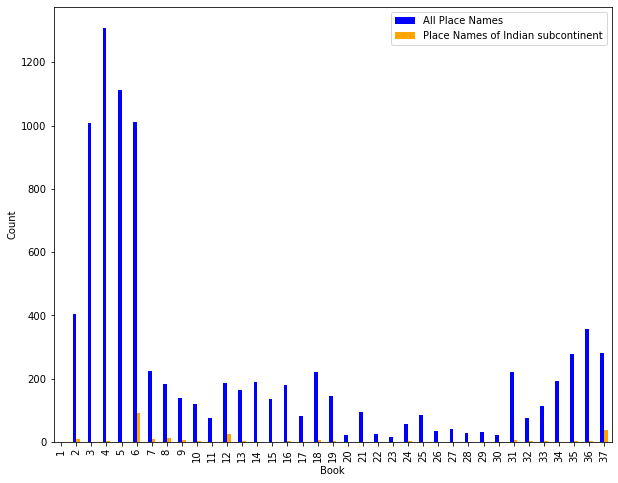
\includegraphics{NHthesis_structure_files/figure-pdf/fig-grouped_place_name_count_comparison-output-1.png}

}

\caption{\label{fig-grouped_place_name_count_comparison}Occurence count
for all place names and place names of Indian subcontinent in each book}

\end{figure}

\begin{figure}

{\centering 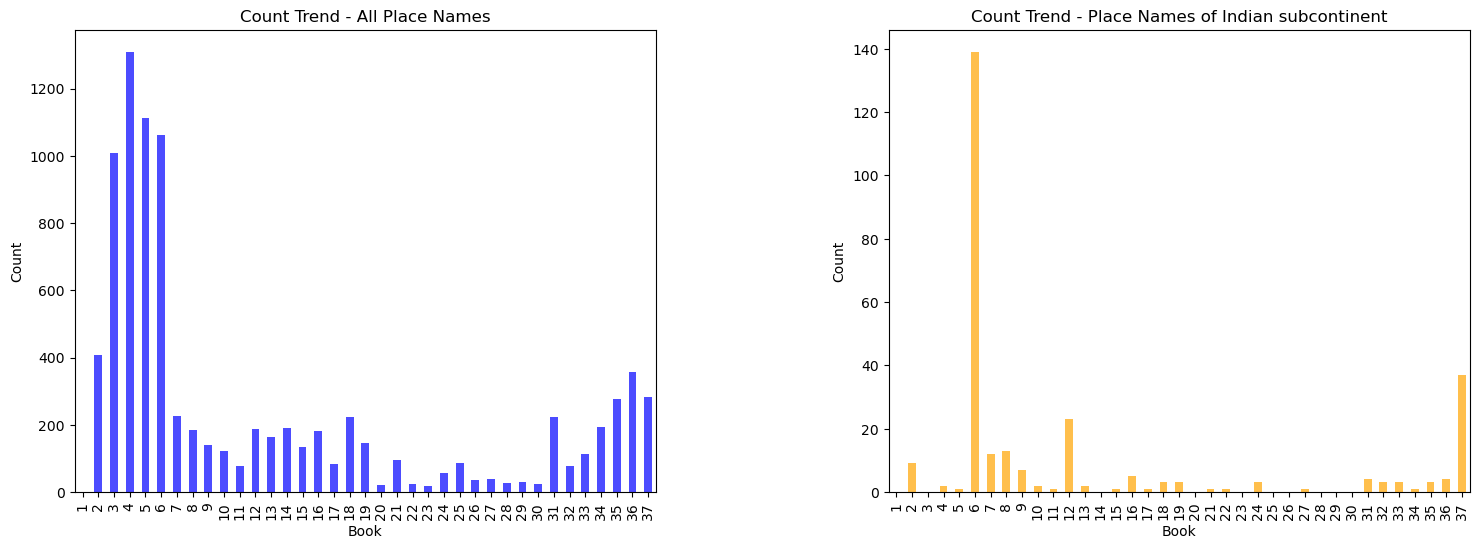
\includegraphics{NHthesis_structure_files/figure-pdf/fig-subplots_place_name_count_comparison-output-1.png}

}

\caption{\label{fig-subplots_place_name_count_comparison}Occurence count
for all place names and place names of Indian subcontinent in each
book\_different y-axis scales}

\end{figure}

The figures reveal a distinct difference between the occurrence trends
of place names related to the Indian subcontinent and all place names
collectively. Specifically, the referencing of the Indian subcontinent
is highly concentrated in books 6, 12, and 37 of Pliny's narrative. This
discrepancy indicates that the mentioning of place names from the Indian
subcontinent is closely tied to specific themes and topics within
Pliny's work.

In this regard, three methodologies have been employed to analyze the
texts pertaining to the Indian subcontinent in \emph{Natural History},
including word frequency and collocation analysis, topic modeling, and
network analysis. The objective of these analyses is to delve deeper
into the textual content, unraveling the intricate relationships and
uncovering the underlying themes and connections associated with the
place names of the Indian subcontinent.

Through word frequency and collocation analysis, the aim is to identify
keyword and significant word combinations co-occur in the textual
content about India in \emph{Natural History}. This analysis provides
insights into the specific linguistic patterns and contextual
associations surrounding the Indian places mentioned in the work,
providing an overview of the keyword in the discourse.

Topic modeling allows for a broader exploration of the thematic
landscape within which the Indian subcontinent place names are embedded.
By clustering related words and identifying prevalent topics, this
methodology helps to discern the major themes and subject matters that
emerge from Pliny's narrative, providing a comprehensive understanding
of the broader context in which these place names are mentioned.

Furthermore, network analysis offers a visual representation of the
interconnections among the place names of the Indian subcontinent and
other entities in Pliny's work. By examining the relationships between
different locations and named entities, this analysis uncovers the
geographical and conceptual networks that exist within the text,
revealing how the Indian subcontinent place names contribute to the
overall structure and narrative flow of \emph{Natural History}.

Together, these methodologies aim to provide a nuanced and comprehensive
exploration of the texts related to the Indian subcontinent in
\emph{Natural History}. By delving into the linguistic, thematic, and
network aspects of these place names, a deeper understanding of their
role in shaping Pliny's narrative can be achieved.

\hypertarget{word-frequency-and-collocating-bi-grams}{%
\subsection{Word frequency and collocating
bi-grams}\label{word-frequency-and-collocating-bi-grams}}

By utilizing the measurements available in the
\href{https://www.nltk.org/}{NLTK} package, a word frequency list and
collocating bi-grams were generated from the text associated with Indian
place names in \emph{Natural History}. These outputs provide an overview
of the prevalent words and word patterns, as potential keywords in the
text.

In the initial observation, the words ``India'' and ``one'' ranked high
in the frequency list. However, it is apparent that the passages would
include the word ``India'' when discussing about India, making it less
informative as a keyword. Likewise, the word ``one'' appeared as a
generic descriptor for bringing up a type of tribe, plant, or attributes
like distance, volume, or range, offering limited insight as a keyword.
To enhance the relevance and descriptive nature of the frequency list,
these two common but less informative words, ``India'' and ``one'', are
further excluded from the token list.

Among 17729 tokens excluding ``India'' and ``one'', 201 (the top 1\%)
frequently occuring words in the India-related text in \emph{Natural
History} are shown in Figure~\ref{fig-freqwords_treemap} and
Figure~\ref{fig-freqwords_wordcloud}.

\begin{figure}

{\centering 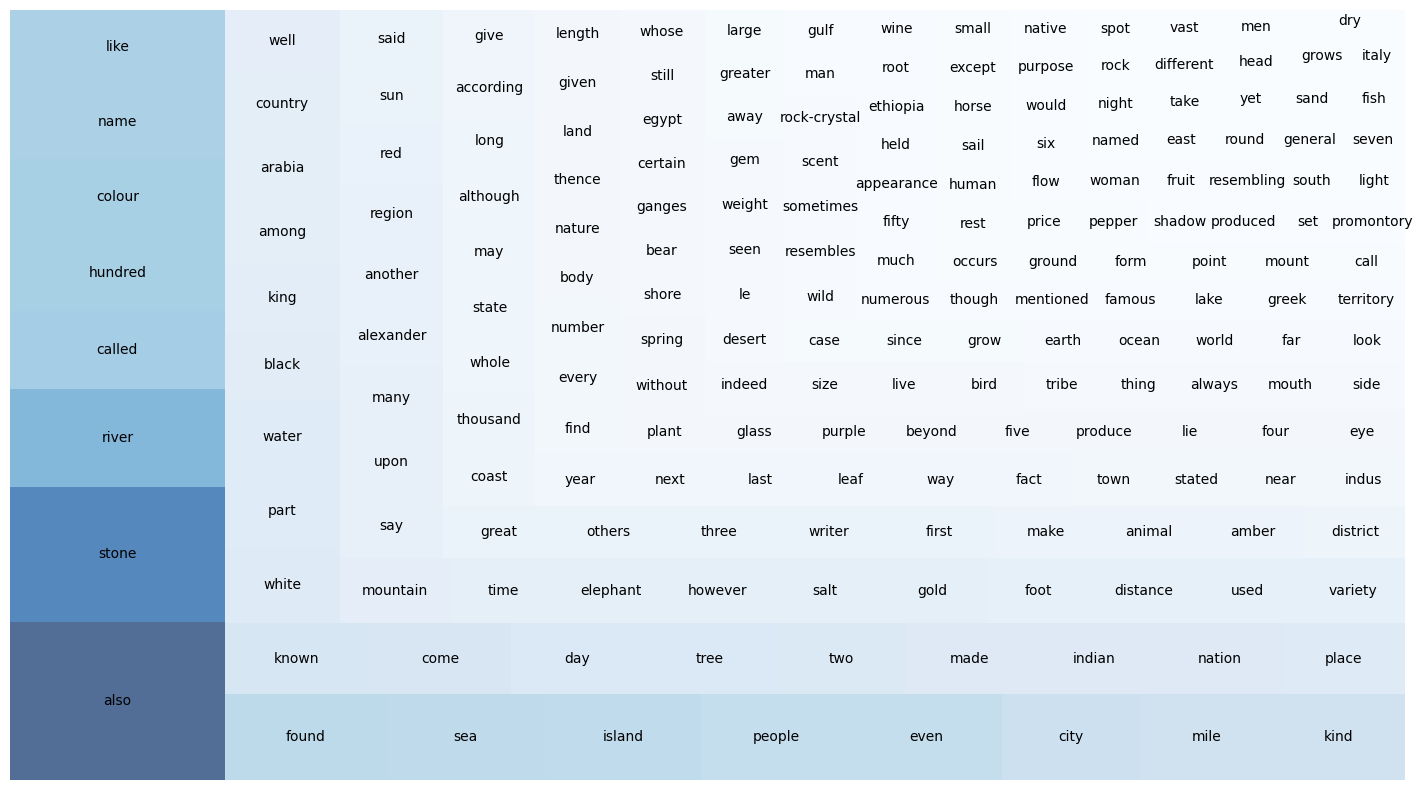
\includegraphics{NHthesis_structure_files/figure-pdf/fig-freqwords_treemap-output-1.png}

}

\caption{\label{fig-freqwords_treemap}Top 1\% frequent words in Indian
subcontinent related text as tree map}

\end{figure}

\begin{figure}

{\centering 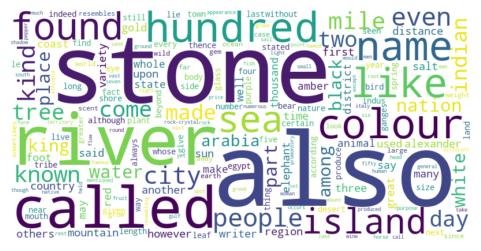
\includegraphics{NHthesis_structure_files/figure-pdf/fig-freqwords_wordcloud-output-1.png}

}

\caption{\label{fig-freqwords_wordcloud}Top 1\% frequent words in Indian
subcontinent related text as word cloud}

\end{figure}

An intriguing observation from the word frequency sorting is the
prominence of the word ``also'' in the given text. The word ``also''
appears frequently, which can be attributed to the encyclopaedic nature
of the work, where it is often used to draw comparisons in introductions
about species and natural phenomena.

As shown in the following examples where ``also'' appears in the
India-related text in \emph{Natural History}, it is indeed used when
comparing the counterparts in India after introducing a natural
phenomenon, plant or human activity. In this regard, the common use of
``also'' may imply that India holds significance as a contrast in the
broader narrative.

\begin{quote}
2.75.1 ``\textbf{Also} in India at the well-known port of Patala the sun
rises\ldots\ldots{}''
\end{quote}

\begin{quote}
12.10.1 ``In India there is \textbf{also} a thorn the wood of which
resembles ebony\ldots\ldots{}''
\end{quote}

\begin{quote}
12.15.1 ``There is \textbf{also} in India a grain resembling that of
pepper, but larger and more brittle\ldots\ldots{}''
\end{quote}

\begin{quote}
12.17.1 ``Arabia \textbf{also} produces cane-sugar, but that grown in
India is more esteemed.''
\end{quote}

The hypothesis is further confirmed towards the end of the work in book
37, where Pliny concludes his comprehensive discourse on ``Nature''. In
37.77.1, Pliny bestows the highest praise upon Italy, considering it to
have earned ``Nature's crown''. And in this context, when expressing his
preference and overall judgment, Pliny makes one final mention of
``India''. He indicates that, ``if we leave aside the fabulous marvels
of India''\footnote{\emph{Natural History} 37.77.1
  (https://topostext.org/work/153)}, Spain can be appreciated as a
significant and attractive destination, second only to Italy. This
unintentional highlight of India suggests that it holds considerable
importance as a distant contrast to the Mediterranean area, where the
focal point locates in the \emph{Natural History}'s world scope.

And following by ``also'', the words ``stone'', ``river'', ``called''
and ``colour'' notably stand out in the word frequeny sorting. These
frequent occurrences suggest some potential themes related to India in
the content of \emph{Natural History}, which aligns with the
distribution of Indian place names as depicted in
Figure~\ref{fig-subplots_place_name_count_comparison}.

Looking into the text in the three books pertaining the most mentions of
Indian place names, book 6 includes specific topics on Nations of India,
the Ganges and Indus (two main rivers in India) and routes of voyages to
India, and book 12 contains introductions to trees and the economic
values of their roots and leaves, as well as plants and their medical
and flavouring effects. While book 37 focuses on descriptions of
different types of gemstones, where the priciple types are introduced in
a sequence/category of colours, alongside critics about the luxury trade
they represents.

The frequent use of the word ``river'' in India-related text may be
related to the mention of voyage and trading routes concerning India in
\emph{Natural History}. On the other hand, ``stone'' and ``color''
clearly connect to the content in book 37, which deals with gemstones.

As indicated by Roller (2022), ``Rivers, especially, were of
significancetotheRomans:Romeoweditsoriginstoitscontrolof a major
crossing of the Tiber that affected travel throughout the Italian
peninsula, and river cults were a major part of Roman ideology''.

These two potential themes observed from the frequent occuring words
indicate that the geographical location and routes toward Indian
subcontinent, and its role as an origin of many plants, animals and
gemstones, pocesses a significance in the content about India in
\emph{Natural History}.

In addition to word frequency observation, collocation analysis is
utilized to explore the common word patterns within the India-related
text in \emph{Natural History}.

The top 0.1\% of the most likely collocating bi-grams are extracted
using the likelihood ratio measurement. This selection process yields 18
out of 17728 bi-grams that are most significant and likely to co-occur
together in the target corpus.

However, during the initial observation, it was noted that approximately
one-third of the extracted bi-grams contained the word ``hundred'', such
as in (`hundred', `fifty') and (`six', `hundred'). These bi-grams
typically denoted measurements for distance, object length, or quantity,
offering limited descriptive information about the content of the text.
Consequently, the word ``hundred'' was excluded from further bi-gram
extraction to focus on more informative and relevant co-occuring words.

And the updated output bi-grams are list as follows:

\begin{verbatim}
[('alexander', 'great'),
 ('father', 'liber'),
 ('caspian', 'gate'),
 ('fifty', 'mile'),
 ('denarii', 'pound'),
 ('gold', 'silver'),
 ('precious', 'stone'),
 ('river', 'indus'),
 ('fourteen', 'equinoctial'),
 ('olive', 'oil'),
 ('asia', 'minor'),
 ('equinoctial', 'hour'),
 ('lapis', 'lazuli'),
 ('red', 'sea'),
 ('mile', 'breadth'),
 ('emperor', 'nero'),
 ('already', 'mentioned'),
 ('ft.', 'long')]
\end{verbatim}

The extracted bi-grams can be broadly categorized into four types:

\textbf{Historical figures}: (`alexander', `great'), (`father',
`liber'), (`emperor', `nero')

\textbf{Geographical locations and features}: (`caspian', `gate'),
(`river', `indus'), (`asia', `minor'), (`red', `sea')

\textbf{Meseuarments (distance, currency, length, time)}: (`fifty',
`mile'), (`denarii', `pound'), (`fourteen', `equinoctial'),
(`equinoctial', `hour'), (`mile', `breadth'), (`ft.', `long')

\textbf{Trading goods}: (`gold', `silver'), (`precious', `stone'),
(`olive', `oil'), (`lapis', `lazuli')

On the one hand, the presence of bi-grams associated with geographical
locations, distance, and time measurements in the India-related text
reaffirms India's position as a geographic reference, consistent with
the earlier findings from the word frequency list and literature review.
On the other hand, within the context of the Indo-Mediterranean network
of exchange, the occurrence of bi-grams related to geographical
locations, currency measurements, and trading goods underscores the
importance of India's role in merchandise trade within the narratives of
\emph{Natural History}.

Furthermore, the occurrence of historical figures such as ``Alexander
III, the Great (king of Macedon)'', ``Nero (Roman emperor)'', and
``Father Liber (referring to Dionysus, the Greek god of winemaking and
wine)'' suggests their connections with India in the history of
expeditions or mythical tales (Dionysus is believed to have conquered
India in Greek epic). This observation opens up a perspective for
clustering the human names mentioned in the text to reveal the content
structure about India in \emph{Natural History}, which will be further
explored in the Network Analysis section.

In conclusion, the analysis of word frequency and collocation in the
India-related text within \emph{Natural History} reveals noteworthy word
patterns. These patterns suggest that India holds a significant role as
a geographical contrast, being compared in terms of distance, natural
phenomena, and origin of products with other regions introduced in the
narrative. Furthermore, it is highlighted for its prominent role in
merchandise trade in the portrait of India in \emph{Natural History}.

\hypertarget{topic-modeling}{%
\subsection{Topic modeling}\label{topic-modeling}}

Furthermore, topic modeling approach is applied to delve further into
the underlying topics about India in the work. Topic modeling is a
widely used method for text analysis that infers the latent topics in a
collection of documents(Bail n.d.; Underwood 2012). Latent Dirichlet
Allocation (LDA), as its most commonly employed algorithm, operates
under an assumption that each document contains a mixture of different
topics, and each topic is defined as a collection of words with varying
probabilities of appearance in the passages(Underwood 2012; Kapadia
2022).

In this study, the collection of India-related text in \emph{Natural
History}, segmented into paragraphs, are considered as different
``documents''. And the \href{https://radimrehurek.com/gensim/}{Genism}
library in Python is utilized for semantic vectorization and the
implementation of the LDA model on the groups of words within the
text\footnote{The code for LDA implementation was referred to the
  tutorial of Barber (n.d.)}.

Since the corpus size for text pertaining to Indian place names is
relatively small, after several attempts with a consideration of the
coherence score distribution depicted in
Figure~\ref{fig-topic_coherence_distribution}, the number of topics is
determined to be 3, with 40 passes to obtain the most optimal and
non-overlapping topic clusters.

\begin{figure}

{\centering 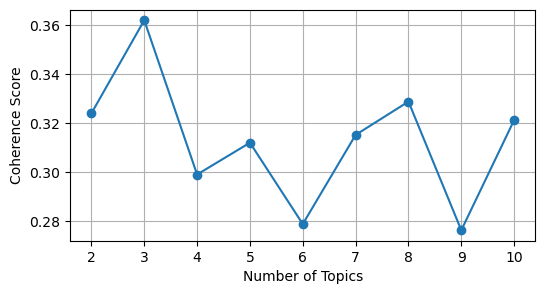
\includegraphics{NHthesis_structure_files/figure-pdf/fig-topic_coherence_distribution-output-1.png}

}

\caption{\label{fig-topic_coherence_distribution}Conherence distribution
of different topic numbers when passes=40}

\end{figure}

And the list of 30 keywords, grouped by the 3 assigned topics, is
presented below.

\begin{verbatim}
[(0,
  '0.014*"stone" + 0.011*"also" + 0.007*"colour" + 0.007*"india" + '
  '0.007*"found" + 0.006*"like" + 0.004*"one" + 0.004*"black" + 0.004*"tree" + '
  '0.004*"amber" + 0.004*"name" + 0.003*"known" + 0.003*"white" + 0.003*"kind" '
  '+ 0.003*"gold" + 0.003*"made" + 0.003*"even" + 0.003*"called" + '
  '0.003*"indian" + 0.003*"glass" + 0.002*"part" + 0.002*"people" + '
  '0.002*"used" + 0.002*"variety" + 0.002*"many" + 0.002*"river" + '
  '0.002*"make" + 0.002*"rock-crystal" + 0.002*"island" + 0.002*"red"'),
 (1,
  '0.009*"stone" + 0.008*"also" + 0.007*"india" + 0.006*"like" + 0.006*"kind" '
  '+ 0.006*"colour" + 0.005*"name" + 0.005*"one" + 0.004*"called" + '
  '0.004*"even" + 0.004*"white" + 0.003*"pepper" + 0.003*"variety" + '
  '0.003*"another" + 0.003*"known" + 0.003*"tree" + 0.003*"black" + '
  '0.003*"weight" + 0.003*"leaf" + 0.003*"purple" + 0.002*"grain" + '
  '0.002*"people" + 0.002*"denarii" + 0.002*"used" + 0.002*"nard" + '
  '0.002*"resembles" + 0.002*"pound" + 0.002*"taste" + 0.002*"found" + '
  '0.002*"small"'),
 (2,
  '0.011*"river" + 0.010*"hundred" + 0.008*"one" + 0.007*"india" + '
  '0.007*"also" + 0.007*"city" + 0.007*"mile" + 0.007*"sea" + 0.006*"island" + '
  '0.005*"nation" + 0.005*"called" + 0.005*"people" + 0.004*"day" + '
  '0.004*"come" + 0.004*"two" + 0.004*"distance" + 0.004*"name" + '
  '0.004*"place" + 0.004*"salt" + 0.004*"king" + 0.003*"elephant" + '
  '0.003*"water" + 0.003*"country" + 0.003*"foot" + 0.003*"alexander" + '
  '0.003*"thousand" + 0.003*"upon" + 0.003*"mountain" + 0.003*"even" + '
  '0.003*"part"')]
\end{verbatim}

Based on the prominent categories of the keywords and the possible
interconnection within each group, a interpretation of the topic emerged
from each keyword clusters can be drawn as follows.

\textbf{Group 0}: This group consists of keywords related to precious
stones, such as ``stone'', ``amber'', ``rock-crystal''and ``glass'',
with colour references like ``black'', ``white'', and ``red''.
Therefore, the underlying topic appears to be the description of
precious stones.

\textbf{Group 1}: This group comprises various natural products, such as
``tree'', ``leaf'', ``pepper'',``grain'' and ``nard'', along with
descriptive words like ``weight'', ``pound'' and ``taste''. In addition,
the ancient Roman currency ``denarii'' appears in the group, suggesting
a possible topic related to merchandise trade with Indian subcontinent.

\textbf{Group 2}: This group contains different geographical features,
such as ``river'', ``island'', ``sea'' and ``mountain''. It also
includes terms related to cities, nations, kings, and distances, and the
name ``Alexander'', referring to Alexander the Great, who has undertook
an expedition to Indian subcontinent. ``Elephant'', as an important
property of the King in India during Pliny's era, also represents the
power and size of the Indian kingdoms. In this regard, the underlying
topic for this group likely pertains to geography and society in India.

The interactive visualisation of the 3 topic clusters, manifesting the
intertopic distance map and the most salient/relevant terms within the
given textand their contributing weights for each topic, can be accessed
on the html version of this
\href{https://raw.githack.com/lizaodawn/NH_thesis/main/NHthesis_structure.html}{thesis}.

The static demonstration of the visualisation can be referred in
Figure~\ref{fig-topic_cluster0}, Figure~\ref{fig-topic_cluster1},
Figure~\ref{fig-topic_cluster2} and Figure~\ref{fig-topic_cluster3}.

The intertopic distance map is shown on the left panel of the
interactive chart. Each bubble represents a topic, and the size of the
bubble indicates the percentage of the texts in the corpus contributing
to the topic. The distance between the bubbles implies the extent of
difference between them. And a good topic model is expected to have big
and non-overlapping bubbles scattered throughout the chart (Tran 2022).

And the most salient/relevant keyword is shown on the right panel. The
blue bars represent the overall frequency of each word in the corpus. If
no topic is selected, the blue bars of the most frequently used words
will be displayed. The contribution of the frequent word to each topic
will be shown in size difference when hovering. And when hovering on the
bubbles in the left panel, there will be red bars in the right panel
giving the estimated number of times a given term was generated by a
given topic. The word with the longest red bar is estimated to be used
the most in the texts belonging to that topic.

\begin{verbatim}
<IPython.core.display.HTML object>
\end{verbatim}

\begin{figure}

{\centering 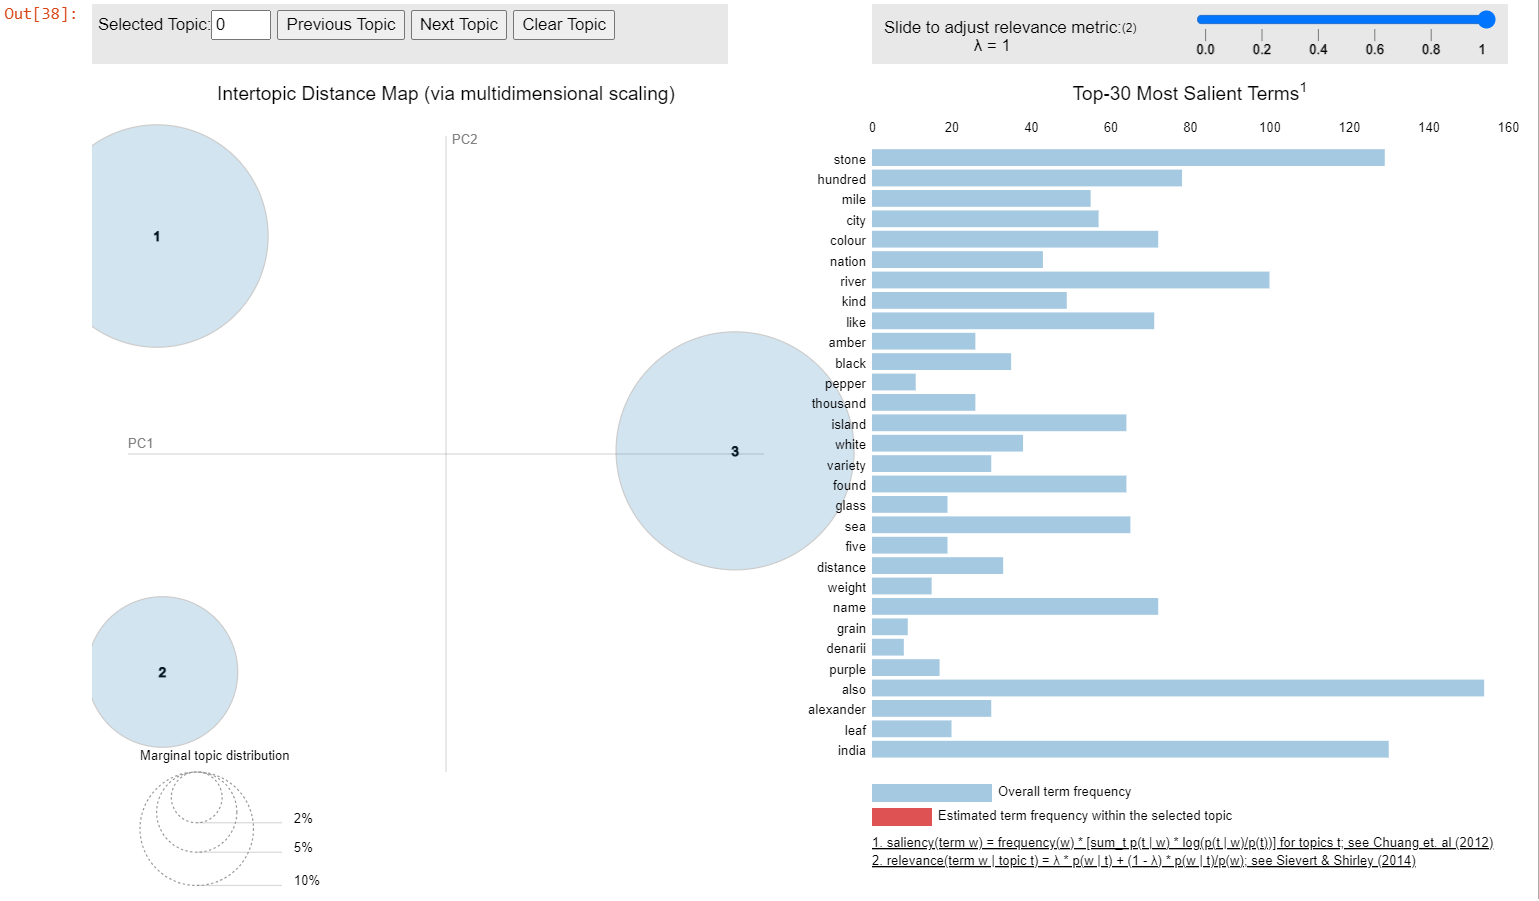
\includegraphics{NHthesis_structure_files/figure-pdf/fig-topic_cluster0-output-1.png}

}

\caption{\label{fig-topic_cluster0}Topic cluster (overall)}

\end{figure}

\begin{figure}

{\centering 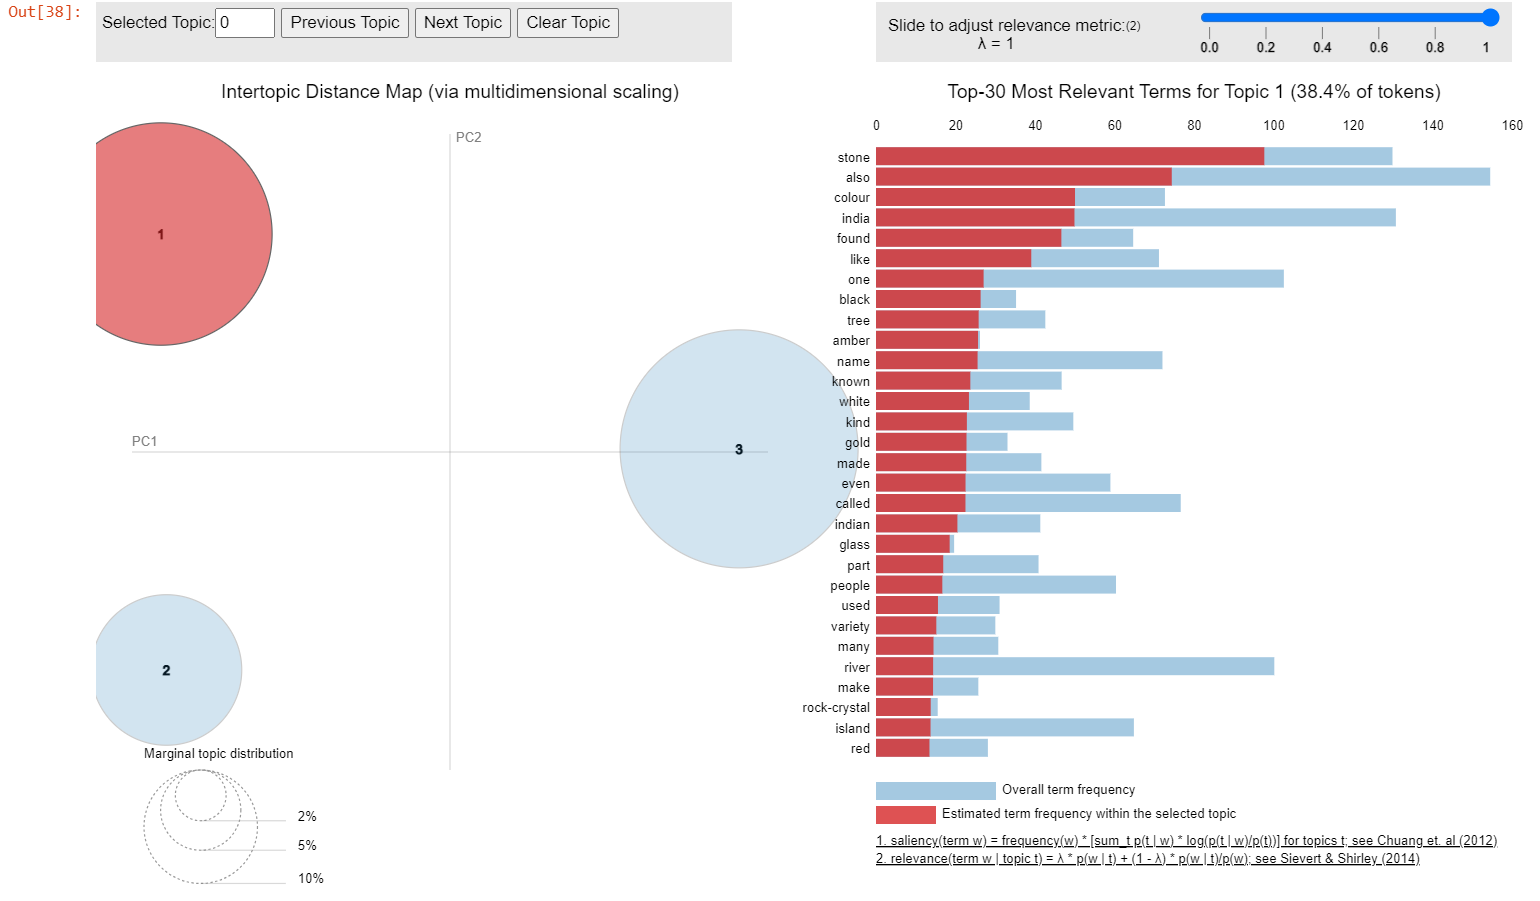
\includegraphics{NHthesis_structure_files/figure-pdf/fig-topic_cluster1-output-1.png}

}

\caption{\label{fig-topic_cluster1}Topic cluster (highlighting on
Topic\_0)}

\end{figure}

\begin{figure}

{\centering 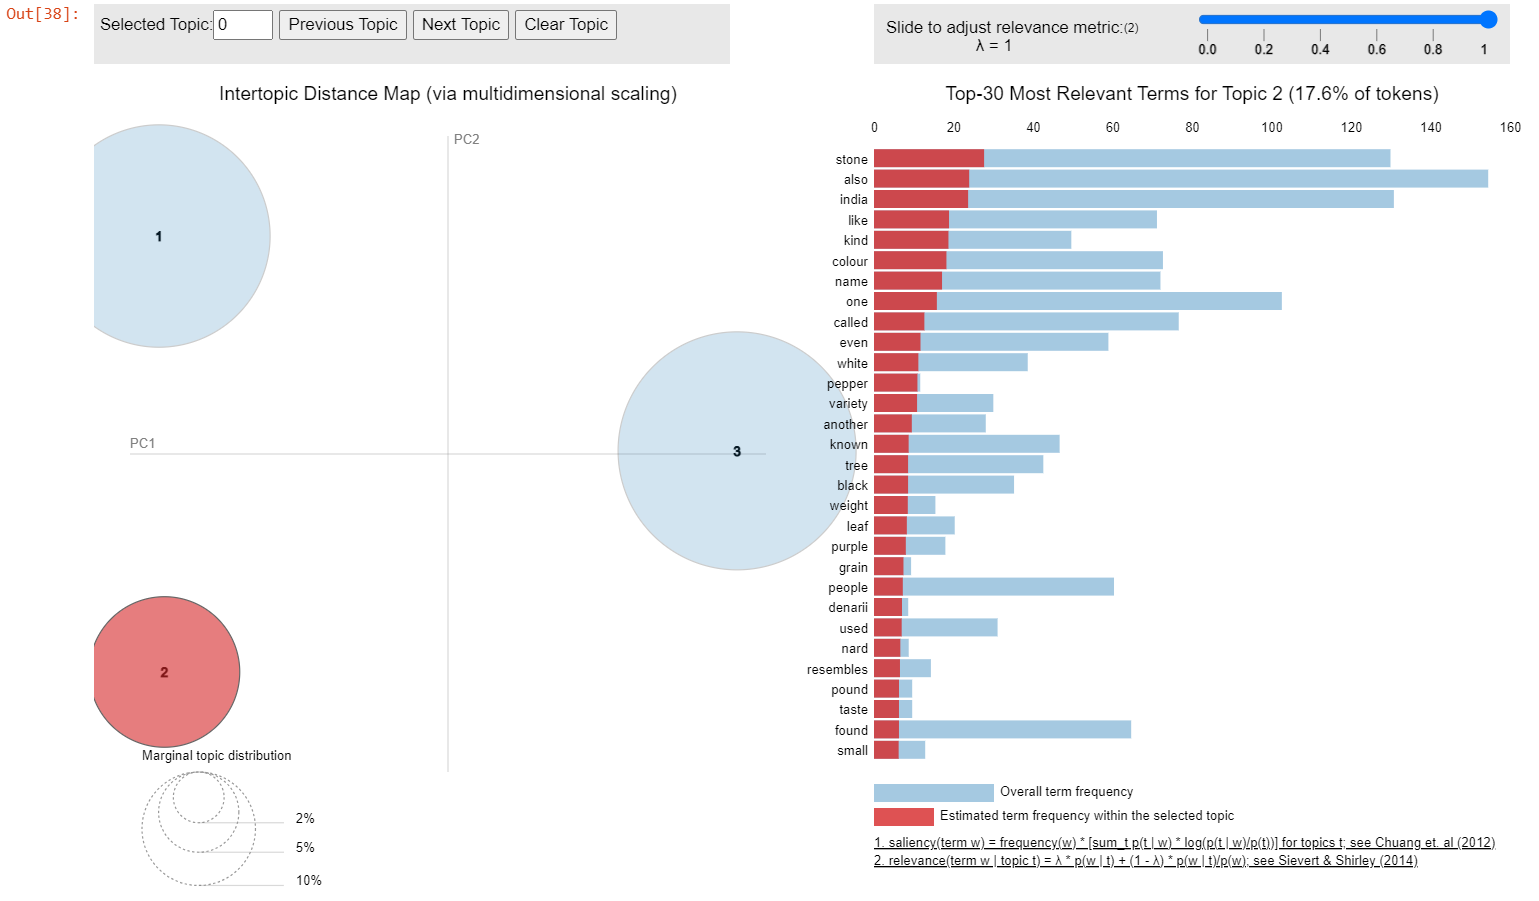
\includegraphics{NHthesis_structure_files/figure-pdf/fig-topic_cluster2-output-1.png}

}

\caption{\label{fig-topic_cluster2}Topic cluster (highlighting on
Topic\_1)}

\end{figure}

\begin{figure}

{\centering 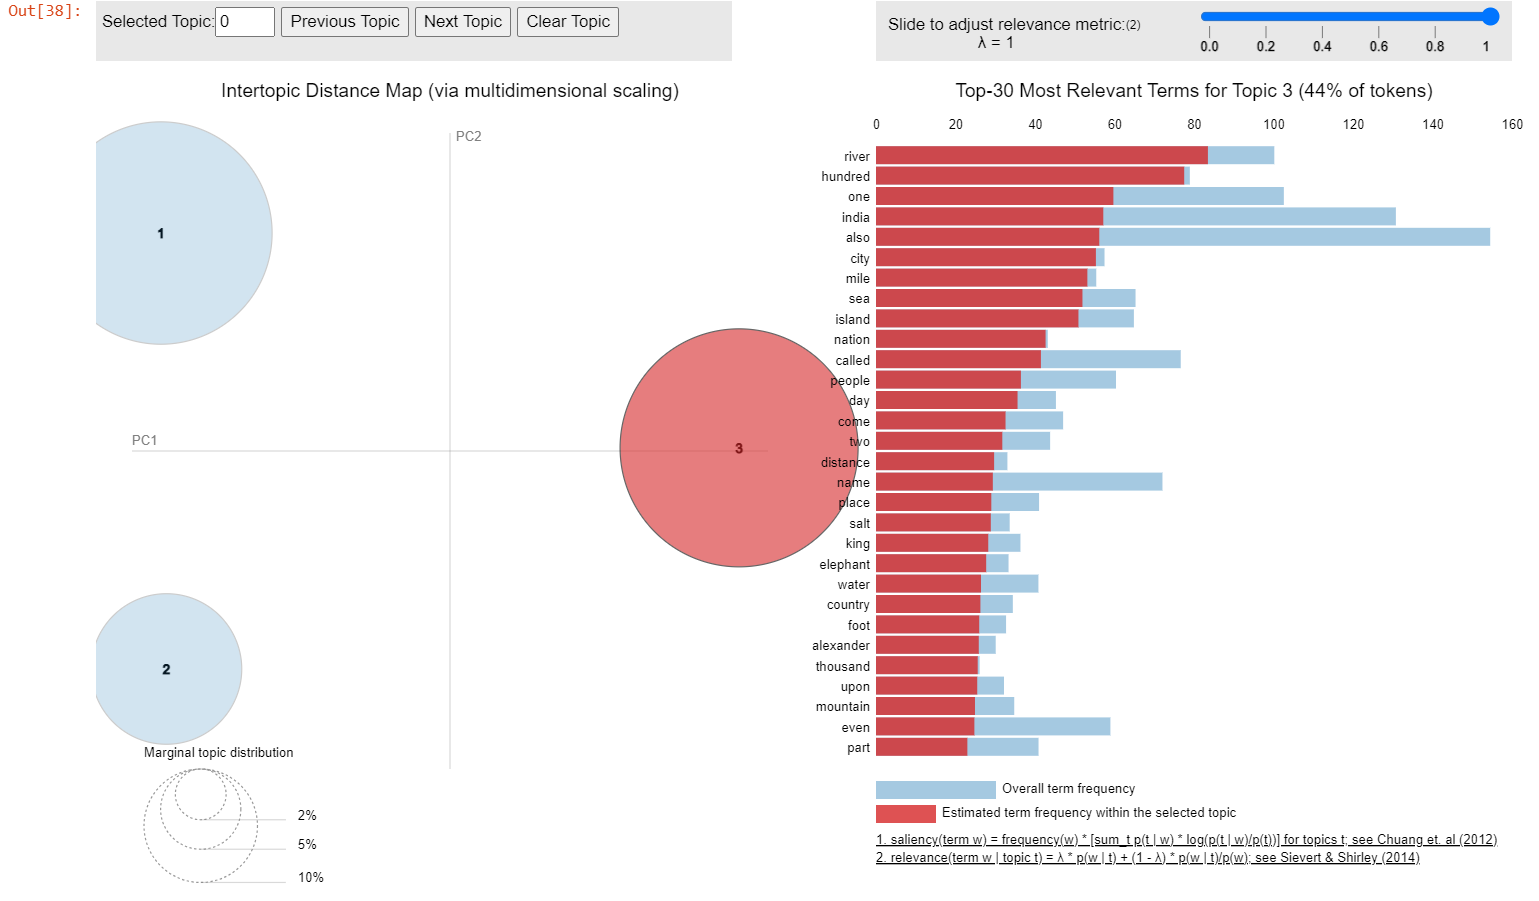
\includegraphics{NHthesis_structure_files/figure-pdf/fig-topic_cluster3-output-1.png}

}

\caption{\label{fig-topic_cluster3}Topic cluster (highlighting on
Topic\_2)}

\end{figure}

In the above visualisation, the three keyword clusters are distanced
from each other, indicating that they formed distinct potential topics
within the given text. And the first (about stones) and the last (about
Indian geography and society) topics took up a more significatnt portion
comparing to the second topic (about merchandise trade).

Additionally, the specific context of the Indian places mentioned in
\emph{Natural History} is manually summarized and categorized into
broader types to serve as a comparison and extension to the topics
generated by the model. The innitial comments about the context were
drawn upon a close reading of the related text, with consideration of
the book and chapter theme indicated in the text. The comments and
summary are stored in CSV format and imported as pandas data frame.

And the summarized comments were further categorized into seven types,
namely {[}`geographical reference', `conquest history', `passing
mention', `general introduction', `criticism', `prominent features',
`goods/animals/plants origin', `producing activity', `product/knowledge
exchange'{]}.

\textbf{Geographical reference}: refers to the occurence of Indian place
names as geographical reference in the narrative, for example:

\begin{quote}
2.112.1 ``\ldots from the river \textbf{Ganges} and its mouth where it
flows into the Eastern Ocean, through \textbf{India} and Parthyene to
the Syrian city of Myriandrus situated on the Issic gulf 5,215\ldots{}''
\end{quote}

\textbf{Passing mention}: refers to the condition that the names of
Indian place included as a side note, for example:

\begin{quote}
5.11.1 ``\ldots Coptos, which from its proximity to the Nile, forms its
nearest emporium for the merchandise of \textbf{India} and
Arabia\ldots{}''
\end{quote}

\textbf{Conquest history}: refers to the mentions of Indian place names
in the context of recalling the conquest history of Alexader the Great,
for example:

\begin{quote}
8.61.2 ``\ldots When Alexander the Great was on his way to
\textbf{India}, the king of Albania had presented him with one dog of
unusually large size\ldots{}''
\end{quote}

\textbf{General introduction}: refers to the focused introduction about
the general situation of places in Indian subcontinent, including
transportation in the work, it is normally directly indicated at the
begining of the affiliated chapter. For example, the whole chapter 21 of
book 6 has a leading topic as ``The nations of India'', the whole
chapter 22 of book 6 has a leading topic as ``The Ganges''.

\textbf{Prominent features}: in \emph{Natural History}, the plants and
animals from India are often noted for their large size, and Pliny often
highlight the good quality of Indian products in his discussion, these
genre of context is categorize as ``prominent features'' of India. For
example:

\begin{quote}
8.14.1 ``\ldots Megasthenes writes that in \textbf{India} snakes grow so
large as to be able to swallow stags and bulls whole\ldots{}'' 37.21.1
``\ldots{}\textbf{India}, likewise, is the sole producer of these stones
and combining, as they do, the brilliant qualities of the most valuable
gems, they above all others description\ldots{}''
\end{quote}

\textbf{Goods/animals/plants origin}: there are also many descriptions
about India as the origin of different goods, animals and plants, this
genre refers to those without concrete comments on their size or
quality, just simply mentioned the object is originated in India, for
example:

\begin{quote}
8.25.2 ``Hyrcania and \textbf{India} produce the tiger, au animal of
terrific speed\ldots{}''
\end{quote}

\textbf{Producing activity}: this genre refer to the cases that
introduces about the human activity or specific producing process about
natural creatures or trading products, such as:

\begin{quote}
8.8.1 ``The method of capturing them in \textbf{India} is for a mahout
riding one of the domesticated elephants\ldots{}'' 37.20.1 ``\ldots The
\textbf{Indians} have found a way of counterfeiting various precious
stones, and beryls in particulars by staining rock-crystal.''
\end{quote}

\textbf{Criticism}: woven in the description about merchandise trade
with Indian subcontinent, Pliny had drwan direct criticism about the
human greed and unnecessary interference on nature it represents, hence
these narratives are specificly grouped together, for example:

\begin{quote}
12.14.2 ``To think that its only pleasing quality is pungency and that
we go all the way to India to get this! Who was the first person who was
willing to try it on his viands, or in his greed for an appetite was not
content merely to be hungry?''
\end{quote}

\begin{quote}
22.56.1 ``I myself shall not touch upon drugs imported from India and
Arabia or from the outer world. Ingredients that grow so far away are
unsatisfactory for remedies\ldots Let them be bought if you like to make
perfumes, unguents and luxuries, or even in the name of religion, for we
worship the gods with frankincense and costmary. But health I shall
prove to be independent of such drugs, if only to make luxury all the
more ashamed of itself.''
\end{quote}

\begin{quote}
33.2.1 ``It came to be deemed the proof of wealth, the true glory of
luxury, to possess something that might be absolutely destroyed in a
moment. Nor was this enough: we drink out of a crowd of precious stones,
and set our cups with emeralds, we take delight in holding India for the
purpose of tippling, and gold is now a mere accessory.''
\end{quote}

\textbf{Product/knowledge exchange}: in some circumstances, Pliny also
mentioned about the knowledge and product exchange during the trade,
such as:

\begin{quote}
34.48.3 ``India possesses neither copper nor lead, and procures them in
exchange for her precious stones and pearls.''
\end{quote}

\begin{quote}
37.23.2 ``\ldots Indeed, as is generally known, in India the stone is
exposed to view by the mountain streams\ldots Later we persuaded the
Indians to share our appreciation of it.''
\end{quote}

And the distribution of context type concluded from close reading is
shown in Figure~\ref{fig-book_context_distribution} and
Figure~\ref{fig-context_type_freq}.

\begin{figure}

{\centering 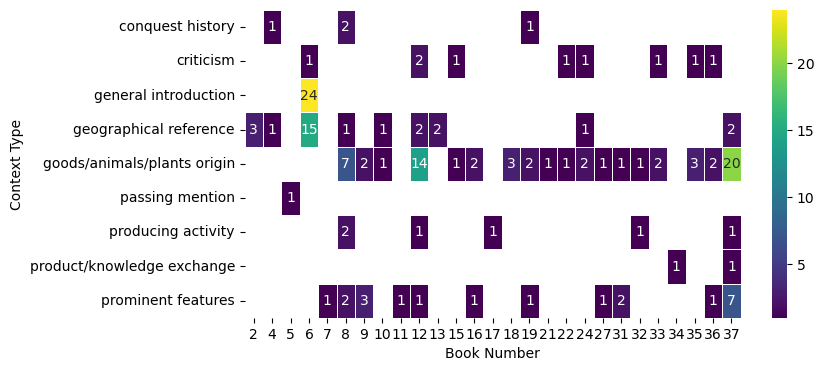
\includegraphics{NHthesis_structure_files/figure-pdf/fig-book_context_distribution-output-1.png}

}

\caption{\label{fig-book_context_distribution}Context type distribution
in books containing Indian place names}

\end{figure}

\begin{figure}

{\centering 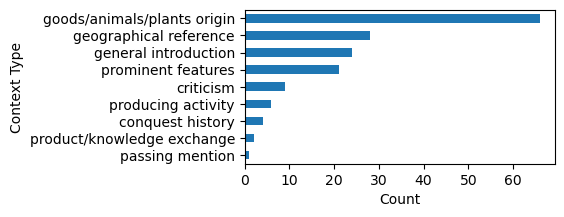
\includegraphics{NHthesis_structure_files/figure-pdf/fig-context_type_freq-output-1.png}

}

\caption{\label{fig-context_type_freq}Occurence frequency of different
context type in India-related text}

\end{figure}

In general, the contexts concluded from the close reading can relate to
the latent topics generated from the distant reading method and added
more details to the keywords clusters. That is, if we understand the
content about India in \emph{Natural History} in three main topics,
namely stons, trade, and contrasting nation, under the ``stone'' topic,
except for describing the colour and texture of different types of
gemstone, there also include the description about India as an origin of
gemstones in a high quality. And under the large proportion of Indian
places as geographical reference and focused introduction mentioned in
the narrative, contributes to the formation of ``nation'' condition as a
major topic. Additionally, there were conquest history of the Roman
Empire to Indian subcontinent referred in the description. And for the
topic about ``trade'', though it seem inferior to the previous two in
terms of quantity, but it is this part that reflects more sentimental
judgement from Pliny out of his stoicism standpoint that worshiping
nature as a devine and against luxurious desire (Beagon 1996).

On top of the observation from the previous section, that India is seen
as an important geographical contrast, as well as a significant trading
partner in the narrative, a more nuanced protrait of India, linking the
conquest story/history of the Roman Empire and criticism aobut human
greed from the stoicism with abundant natural wonders and products of
the best quality in the world can be drawn from the comprehension of
topic modelling and close reading.

\hypertarget{network-analysis-for-named-entity}{%
\subsection{Network analysis for Named
Entity}\label{network-analysis-for-named-entity}}

In addition to the previous methods partly answered on the question
about ``how India is described?'' in \emph{Natural History}, a network
analysis of the named entities in the text may shed a light on the
structure of the India-related content in the work. As inspired by the
person name collocations observed from the collocation analysis, the
initial idea for this section is to extract person names mentioned in
the India-related text, and generate a entity cluster for the person
names, place names, and book number, to explore how the content is
structured in the context.

Employing the dataset with supplemented Indian place name annotations,
distinct place names (including annotated places outside Indian
subcontinenet), person names and book numbers are considered as nodes,
and the co-occurences of person name and place names, as well as that of
two different place names in the same paragraph, and the book number the
person and place name occured, are counted as edges.

To identify the the impact of different entities in the discourse, the
betweeness centrality of the nodes are mesured and represented by the
size of the node. And the weight of edge between two nodes represents
the time the two entities appeared in the same context. Gone through a
Force Atlas 2 layout algorithm, the graph also demonstrates the rough
cluster of entities which tend to be mentioned together.

Indexing with the book-chapter-paragraph number of the India-related
text, the place names outside Indian subcontinent mentioned in the same
paragraph are also included for the network analysis. And according to
the original TOPOSText and supplemented place name annotations, there
are total of 908 occurences of place names in paragraphs of
Indian-related text in \emph{Natural History}.

\hypertarget{person-name-annotationtag-retrieve}{%
\subsubsection{Person name annotation/tag
retrieve}\label{person-name-annotationtag-retrieve}}

In order to extract the people names within the captioned text,
approaches of retriving from the TOPOSText annotation and from the
tagging of text given by the pretrained multilingual named entity
recognition model
\href{https://huggingface.co/Babelscape/wikineural-multilingual-ner}{WikiNEuRal}
(Tedeschi et al. 2021) and
\href{https://huggingface.co/flair/ner-english-ontonotes-fast}{Flair}
(Akbik, Blythe, and Vollgraf 2018) are compared for adopting the most
completed output.

\textbf{1. Annotation retrieving from TOPOSText}

On TOPOSText, other than place names, a list of proper names (including
people, gods, festivals, animals and artworks) are also annotated to the
text of the classics. Each proper name has a unique URI as identifier in
the html structure, such as: **\textless a href=``/people/54''
target=``\_blank''\textgreater Muses\textless/a\textgreater**.

Utilizing the tools of
\href{https://www.crummy.com/software/BeautifulSoup/bs4/doc/}{Beautiful
Soup}, the textual proper names, their URIs along with the
book-chapter-paragraph number they occured in, can be retrieved with the
URLs of both parts of \emph{Natural History} on TOPOSText.

In the annotated text of \emph{Natural History} on TOPOSText, there are
5109 such proper name annotations in book 1-11 and 7038 in book 12-37,
adding up to a combined total of 12147 throughout the work.

The specific annotation type as ``person name'' can be further validated
with the \href{https://topostext.org/api/people/readweb.php}{api} on
TOPOText. In the api file, all the entities of people/gods, has been
valued as ``male'' or ``female'' as its ``gender'' key. Based on this
criteria, those with other values in their ``gender'' key, such as
``gender'':``animal'' or ``gender'':``other'', are not considered as
``people'' and filtered out from the retrieved output. Moreover, as
there is a ``concat'' value indicating a detailed name of the signified
person and shared with all variants of the same URI, the ``concat''
value is also fetched as a more accurate information of person name
enetity.

\hypertarget{tbl-validated_people_anno}{}
\begin{longtable}[]{@{}llllll@{}}
\caption{\label{tbl-validated_people_anno}Example of retrieved and
validated person name annotations in \emph{Naturl
History}}\tabularnewline
\toprule\noalign{}
& FILE\_ID & Person\_name & ToposText\_ID & Reference &
Person\_name\_concat \\
\midrule\noalign{}
\endfirsthead
\toprule\noalign{}
& FILE\_ID & Person\_name & ToposText\_ID & Reference &
Person\_name\_concat \\
\midrule\noalign{}
\endhead
\bottomrule\noalign{}
\endlastfoot
0 & 1.1.1 & Muses & /people/54 & urn:cts:latinLit:phi0978.phi001:1.1.1 &
Muses (goddesses) \\
1 & 1.1.1 & Catullus & /people/1881 &
urn:cts:latinLit:phi0978.phi001:1.1.1 & Catullus \\
2 & 1.2.1 & Cicero & /people/2300 &
urn:cts:latinLit:phi0978.phi001:1.2.1 & Marcus Tullius Cicero \\
3 & 1.2.1 & Cicero & /people/2300 &
urn:cts:latinLit:phi0978.phi001:1.2.1 & Marcus Tullius Cicero \\
4 & 1.2.1 & Manius & /people/382 & urn:cts:latinLit:phi0978.phi001:1.2.1
& Manius \\
\end{longtable}

An example of the data structure of the retrieved output of person name
annotations in \emph{Natural History} is shown in
Table~\ref{tbl-validated_people_anno}. There are total 6568 occurences
of person names annotated in the whole work, \textbf{330} of which are
within the India-related text.

\hypertarget{tbl-person_anno_merged}{}
\begin{longtable}[]{@{}llllll@{}}
\caption{\label{tbl-person_anno_merged}Example for person name
annotation merged into India-related text dataset}\tabularnewline
\toprule\noalign{}
& FILE\_ID & Place\_Name & Book & Text & Person\_name\_concat \\
\midrule\noalign{}
\endfirsthead
\toprule\noalign{}
& FILE\_ID & Place\_Name & Book & Text & Person\_name\_concat \\
\midrule\noalign{}
\endhead
\bottomrule\noalign{}
\endlastfoot
0 & 2.75.1 & Syene & 2.0 & Similarly it is reported that at the town of
S... & Onesicritus \\
1 & 2.75.1 & Syene & 2.0 & Similarly it is reported that at the town of
S... & Alexander III, the Great (general) \\
2 & 2.75.1 & Syene & 2.0 & Similarly it is reported that at the town of
S... & Alexander III, the Great (general) \\
3 & 2.75.1 & Syene & 2.0 & Similarly it is reported that at the town of
S... & Onesicritus \\
4 & 2.75.1 & India & 2.0 & Similarly it is reported that at the town of
S... & Onesicritus \\
\end{longtable}

As shown in Table~\ref{tbl-person_anno_merged}, the validated annotated
person names are added to the India-related text dataset. With the
person name annotation retrieving, there found total \textbf{3583}
co-occurences of single place name and person name in the same paragraph
within the India-related text in \emph{Natural History}.

\textbf{2. Named entity recognition with
\href{https://huggingface.co/Babelscape/wikineural-multilingual-ner}{WikiNEuRal}}

To evaluate the quality and completeness of the extracted person name
annotations, two widely practiced pretrained machine learning models for
named entity recognition,
\href{https://huggingface.co/Babelscape/wikineural-multilingual-ner}{WikiNEuRal}
(Tedeschi et al. 2021) and
\href{https://huggingface.co/flair/ner-english-ontonotes-fast}{Flair}
(Akbik, Blythe, and Vollgraf 2018) are utilized for tagging person names
in the India-related text.

\hypertarget{tbl-wiki_ppl_tag}{}
\begin{longtable}[]{@{}lllll@{}}
\caption{\label{tbl-wiki_ppl_tag}Example of person name tags retrieved
with WikiNEuRal from India-related text in \emph{Natural
History}}\tabularnewline
\toprule\noalign{}
& FILE\_ID & Text & Text\_ner & PER\_name\_tag \\
\midrule\noalign{}
\endfirsthead
\toprule\noalign{}
& FILE\_ID & Text & Text\_ner & PER\_name\_tag \\
\midrule\noalign{}
\endhead
\bottomrule\noalign{}
\endlastfoot
0 & 2.75.1 & Similarly it is reported that at the town of S... &
{[}\{\textquotesingle entity\_group\textquotesingle:
\textquotesingle LOC\textquotesingle,
\textquotesingle score\textquotesingle: 0.99636984, ... & Onesicritus \\
0 & 2.75.1 & Similarly it is reported that at the town of S... &
{[}\{\textquotesingle entity\_group\textquotesingle:
\textquotesingle LOC\textquotesingle,
\textquotesingle score\textquotesingle: 0.99636984, ... & Alexander \\
0 & 2.75.1 & Similarly it is reported that at the town of S... &
{[}\{\textquotesingle entity\_group\textquotesingle:
\textquotesingle LOC\textquotesingle,
\textquotesingle score\textquotesingle: 0.99636984, ... & Alexander \\
0 & 2.75.1 & Similarly it is reported that at the town of S... &
{[}\{\textquotesingle entity\_group\textquotesingle:
\textquotesingle LOC\textquotesingle,
\textquotesingle score\textquotesingle: 0.99636984, ... & Onesicritus \\
21 & 2.112.1 & Our own portion of the earth, which is my subj... &
{[}\{\textquotesingle entity\_group\textquotesingle:
\textquotesingle LOC\textquotesingle,
\textquotesingle score\textquotesingle: 0.7412269, \textquotesingle... &
Artemidorus \\
\end{longtable}

An example of the person name tags retrieved from WikiNEuRal of the
given text are shown in Table~\ref{tbl-wiki_ppl_tag}. There are total
\textbf{225} occurences retrieved within the India-related text.

And after merging the person name tags with the dataset of place name
occurences, there found total \textbf{1881} co-occurences of single
place name and person name in the same paragraph within the
India-related text in \emph{Natural History}.

\textbf{3. Named entity recognition with
\href{https://huggingface.co/flair/ner-english-ontonotes-fast}{Flair}}

As a comparison, another well-esteemed NLP pretrained model,
\href{https://huggingface.co/flair/ner-english-ontonotes-fast}{Flair}
(Akbik, Blythe, and Vollgraf 2018) is also applied for the named enetity
recognition to the same text.

\hypertarget{tbl-flair_ppl_tag}{}
\begin{longtable}[]{@{}lllll@{}}
\caption{\label{tbl-flair_ppl_tag}Example of person name tags retrieved
with Flair from India-related text in \emph{Natural
History}}\tabularnewline
\toprule\noalign{}
& FILE\_ID & Text & Text\_ner & PER\_name\_tag \\
\midrule\noalign{}
\endfirsthead
\toprule\noalign{}
& FILE\_ID & Text & Text\_ner & PER\_name\_tag \\
\midrule\noalign{}
\endhead
\bottomrule\noalign{}
\endlastfoot
0 & 2.75.1 & Similarly it is reported that at the town of S... &
{[}\{\textquotesingle entity\_group\textquotesingle:
\textquotesingle LOC\textquotesingle,
\textquotesingle score\textquotesingle: 0.99636984, ... & Leo \\
0 & 2.75.1 & Similarly it is reported that at the town of S... &
{[}\{\textquotesingle entity\_group\textquotesingle:
\textquotesingle LOC\textquotesingle,
\textquotesingle score\textquotesingle: 0.99636984, ... & Alexander \\
0 & 2.75.1 & Similarly it is reported that at the town of S... &
{[}\{\textquotesingle entity\_group\textquotesingle:
\textquotesingle LOC\textquotesingle,
\textquotesingle score\textquotesingle: 0.99636984, ... & Alexander \\
0 & 2.75.1 & Similarly it is reported that at the town of S... &
{[}\{\textquotesingle entity\_group\textquotesingle:
\textquotesingle LOC\textquotesingle,
\textquotesingle score\textquotesingle: 0.99636984, ... & Onesicritus \\
66 & 4.17.4 & Such is Macedonia, which was once the mistress... &
{[}\{\textquotesingle entity\_group\textquotesingle:
\textquotesingle LOC\textquotesingle,
\textquotesingle score\textquotesingle: 0.95384216, ... & Paulus
Aemilius \\
\end{longtable}

An example of the person name tags retrieved from WikiNEuRal of the
given text are shown in Table~\ref{tbl-flair_ppl_tag}. There are total
\textbf{102} occurences retrieved within the India-related text.

And after merging the person name tags with the dataset of place name
occurences, there found total \textbf{938} co-occurences of single place
name and person name in the same paragraph within the India-related text
in \emph{Natural History} with the NER tool of Flair.

As shown in Table~\ref{tbl-ner_compare}, the TOPOSText annotation
provide more person name entities comparing to the other two methods.

\hypertarget{tbl-ner_compare}{}
\begin{longtable}[]{@{}llll@{}}
\caption{\label{tbl-ner_compare}Quantity of person name entities
retrieved with different methods}\tabularnewline
\toprule\noalign{}
& Distinct person name & Person name occurence & Place-person
co-occurence \\
\midrule\noalign{}
\endfirsthead
\toprule\noalign{}
& Distinct person name & Person name occurence & Place-person
co-occurence \\
\midrule\noalign{}
\endhead
\bottomrule\noalign{}
\endlastfoot
TOPOSText Annotation & 153 & 330 & 3583 \\
WikiNEuRal NER & 121 & 225 & 1881 \\
Flair NER & 71 & 102 & 938 \\
\end{longtable}

And the first fifteen distinct retrieved person names of the three
methods can be referred in Table~\ref{tbl-per_name_compare}. For the
case of ``Alexander III, the Great (general)'', since the annotation
retrieved from TOPOSText is validated with the URI, both ``Alexander''
and ``Alexander the Great'' will be recognized as the same entity. While
from the output of WikiNEuRal and Flair, the two variants are recognized
as two different entities. And for the case ``Leo'' retrieved from Flair
NER, it actually refers to the zodiac constellation, rather than a
person/god name, and the same entity has a ``gender'':``astronomic''
value in the TOPOSText annotation, which will prevent it being added to
the dataset as a person name.

\hypertarget{tbl-per_name_compare}{}
\begin{longtable}[]{@{}llll@{}}
\caption{\label{tbl-per_name_compare}First 15 distinct person names
retrieved with different methods}\tabularnewline
\toprule\noalign{}
& TOPOSText Annotation & WikiNEuRal NER & Flair NER \\
\midrule\noalign{}
\endfirsthead
\toprule\noalign{}
& TOPOSText Annotation & WikiNEuRal NER & Flair NER \\
\midrule\noalign{}
\endhead
\bottomrule\noalign{}
\endlastfoot
0 & Onesicritus & Onesicritus & Leo \\
1 & Alexander III, the Great (general) & Alexander & Alexander \\
2 & Heracles (s. of Zeus), Hercules & Artemidorus & Onesicritus \\
3 & Artemidorus Ephesius & Isidore & Paulus Aemilius \\
4 & Isidoros of Charax & Father Liber & Cyrus \\
5 & Dionysus (s. of Zeus), Bacchus & Hercules & SCYTHIA \\
6 & Paulus & Paulus Aemilius & Aramii \\
7 & Aemilius & Amasis & M. Varro \\
8 & Amasis & Alexander the Great & Pompey \\
9 & Memnon (s. of Tithonus) & Antiochus & Laros \\
10 & Osiris & Seleucus & Hecataeus \\
11 & Calliope (d. of Zeus) & M & Patrocles \\
12 & Antiochus, Antiochos (misc) & Varro & Alexander the Great \\
13 & Seleucus I Nicator s. Antiochus & Amometus & Baeton \\
14 & Margos & Hecataeus & Protalis \\
\end{longtable}

Both in terms of quantity and quality, the person names retrieved from
the TOPOSText is more reliable for this study. Therefore, the output of
TOPOSText annotation retriving is appended to the dataset for node/edge
generation for the network analysis.

\hypertarget{network-graph-generation}{%
\subsubsection{Network graph
generation}\label{network-graph-generation}}

As mentioned, there will be three types of nodes for the expected
network graph, namely \textbf{place name}, \textbf{person name} and
\textbf{book number}.

And there are four types of edges taken into consideration, including
the co-occurence of:

\begin{enumerate}
\def\labelenumi{\arabic{enumi}.}
\tightlist
\item
  \textbf{place name} and \textbf{person name} in the same paragraph
\item
  \textbf{person name} and \textbf{book number} it appears in
\item
  \textbf{place name} and \textbf{book number} it appears in
\item
  \textbf{place name} and \textbf{place name} in the same paragraph
\end{enumerate}

There are total 519 nodes and 14177 edges for the network of place
name/person name/book number in India-related text of \emph{Natural
History}.

The network graph generated from the captioned nodes and edges can be
explored as Figure~\ref{fig-network_graph}. The size of the nodes
represents the betweeness centralality of the entity in the context,
which means the bigger the node, the more central it is in the
discourse. The types of nodes (place name, person name, book number) are
differenciated by colour.

And the curved lines linking different nodes indicate the co-occurences
between single place name and person name, two place names, and the book
number of place name and person name occurs. The thickness of the line
represent the counts of the co-occurence edge, which means, the thicker
the line linking, the more frequent the two nodes are mentioned
together.

Apparently, ``India'' is the absolute center of the discourse. And
drawing from both the node size and edge thickness, ``Arabia'' is the
place that often mentioned together with India. Actually, the two
countries are often mentioned in the same time, for example:

\begin{quote}
13.28.1 ``Ethiopia, which is on the borders of Egypt, has virtually no
remarkable trees except the wool-tree, like the one described among the
trees of \textbf{India} and \textbf{Arabia}.''
\end{quote}

\begin{quote}
22.56.1 ``I myself shall not touch upon drugs imported from
\textbf{India} and \textbf{Arabia} or from the outer world.''
\end{quote}

One possible reason for this pairing occurence is that Arabia locates in
the middle of the route from Rome to India, and the two places similarly
are significant importers for the exotic and luxurious goods trade.

\begin{figure}

{\centering 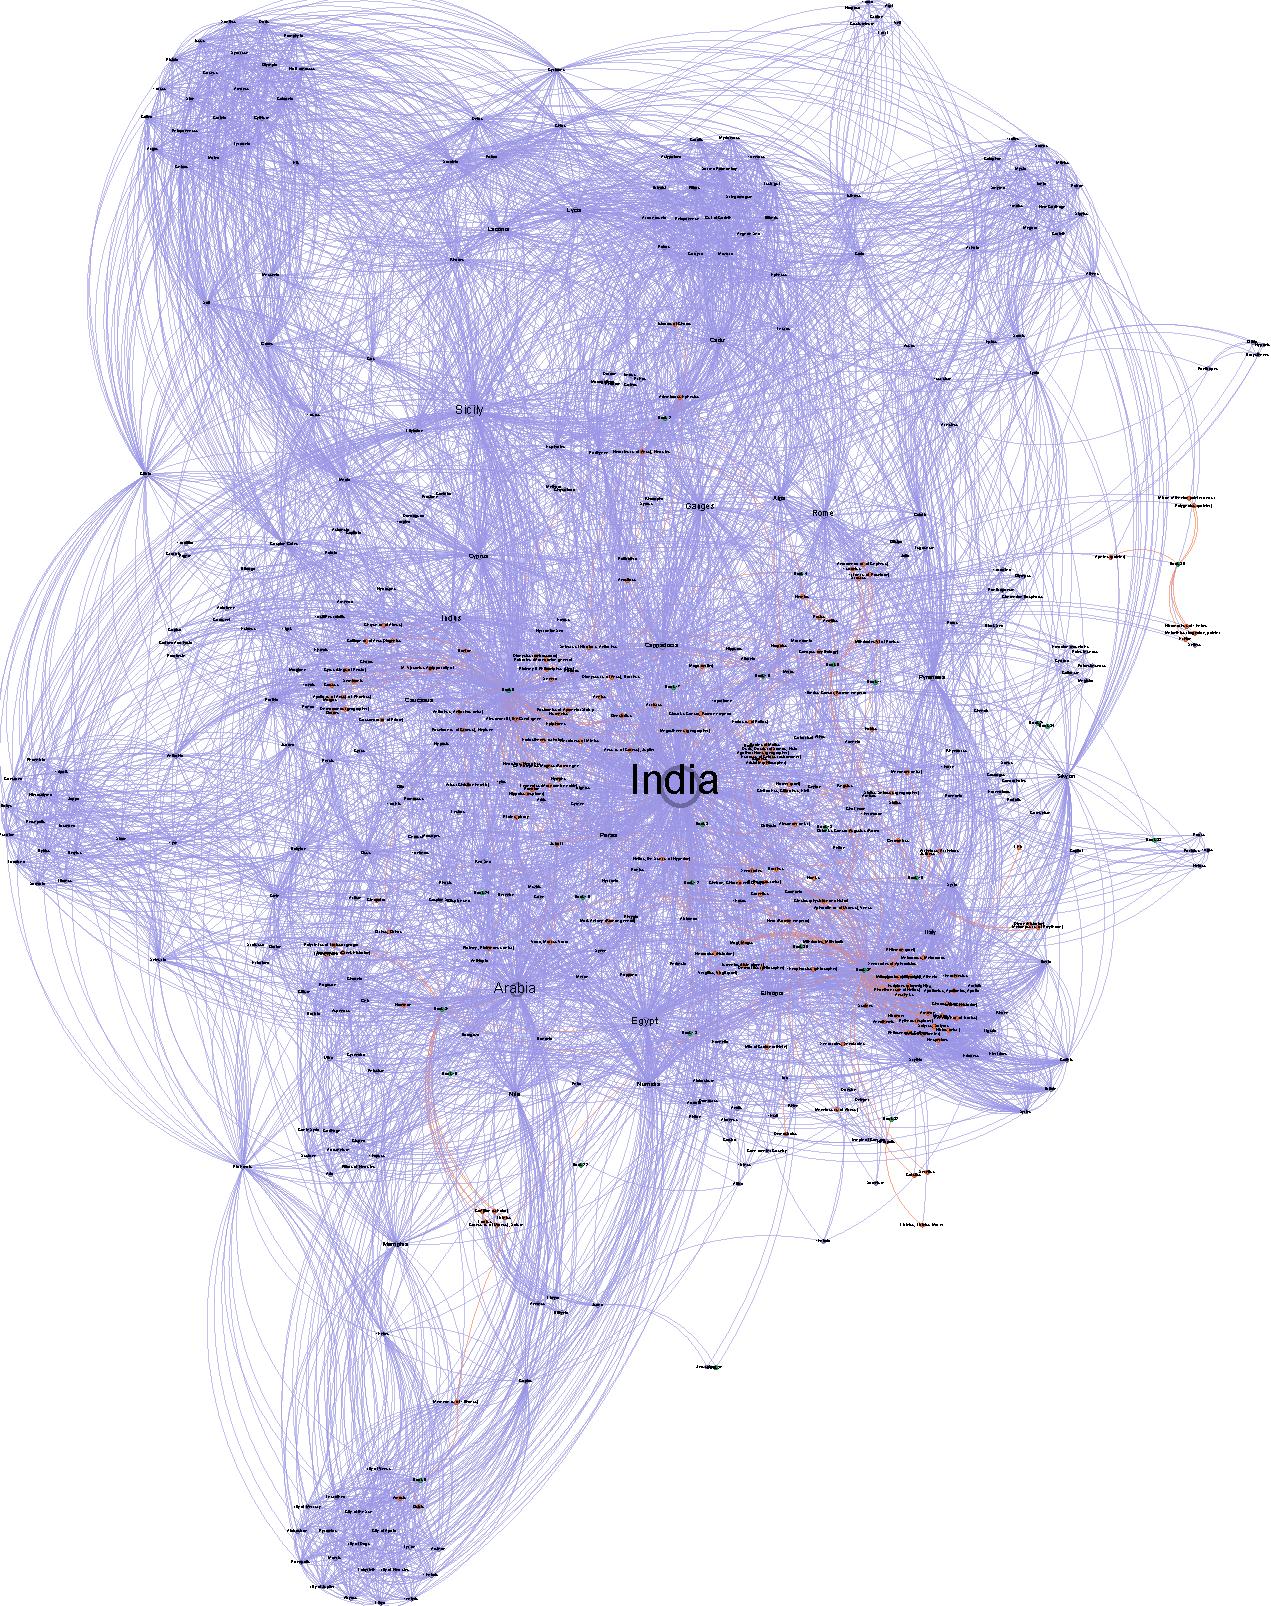
\includegraphics{NHthesis_structure_files/mediabag/NHthesis_structure_files/figure-pdf/fig-network_graph-output-1.pdf}

}

\caption{\label{fig-network_graph}Place/person/book number network of
India-related content in \emph{Natural History}}

\end{figure}

Besides, there are several groups of place names located the edge of the
graph, as shown in Figure~\ref{fig-nw_edged_groups}, indicating they
tend to be mentioned together, but relatively distanced from the
discussion of India. In most cases India is just a passing metion in the
enumerition context.

\begin{figure}

{\centering 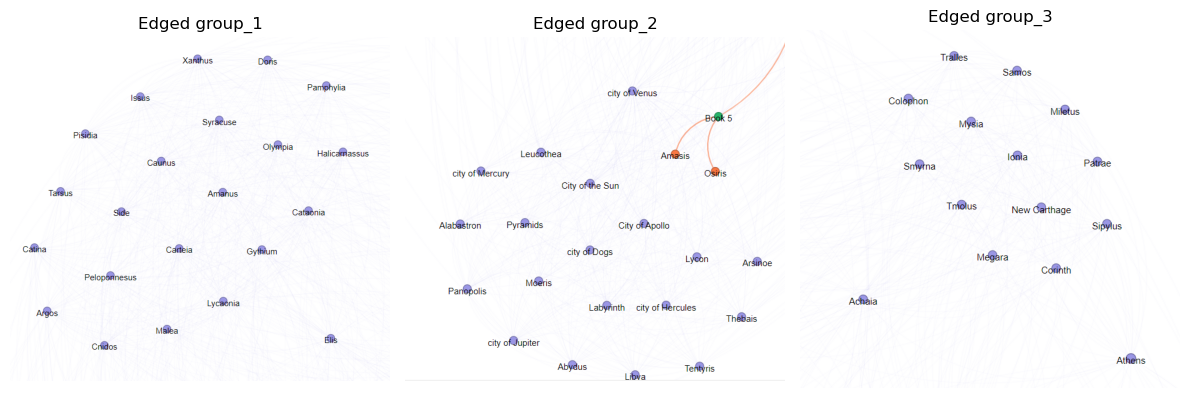
\includegraphics{NHthesis_structure_files/figure-pdf/fig-nw_edged_groups-output-1.png}

}

\caption{\label{fig-nw_edged_groups}Example of edged groups in the
network graph of India-related text in \emph{Natural History}}

\end{figure}

And there are three obvious person name clusters centering on Book 6,
Book 7 and Book 37, the zoomed in captures are shown in
Figure~\ref{fig-network_zoom_book6n7} (for Book 6 and Book 7) and
Figure~\ref{fig-network_zoom_book37} (for Book 37).

\begin{figure}

{\centering 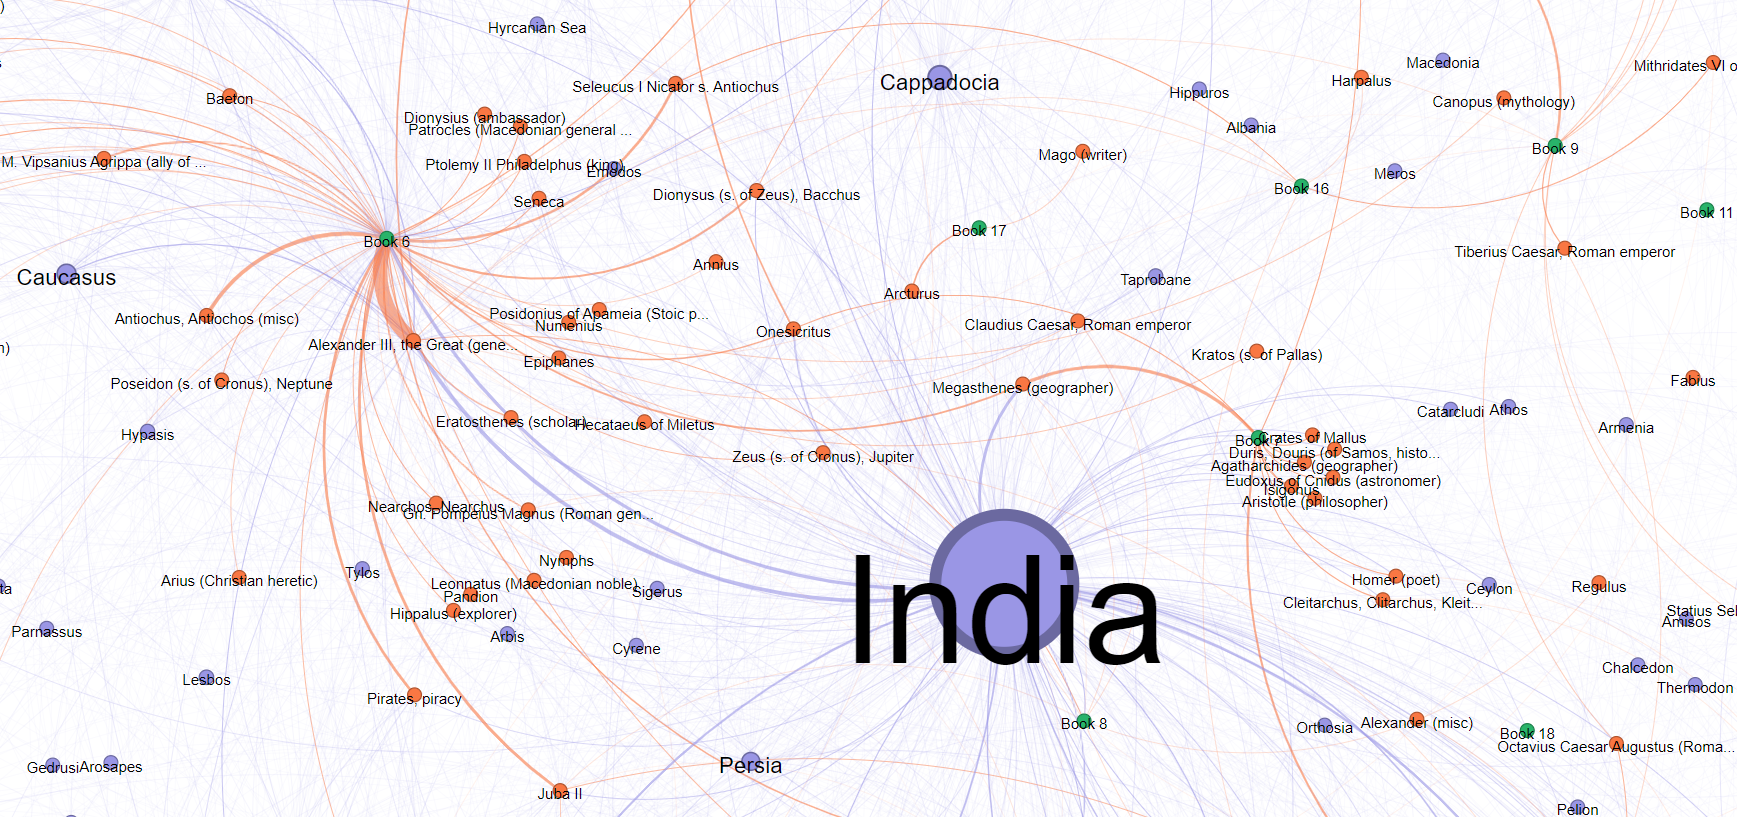
\includegraphics{NHthesis_structure_files/figure-pdf/fig-network_zoom_book6n7-output-1.png}

}

\caption{\label{fig-network_zoom_book6n7}Clusters of Book 6 \& Book 7 in
India-related content in \emph{Natural History}}

\end{figure}

From the cluster of Book 6, the most frequent mentioned historical
figures are Alexander the Great and Dionysus (often with a variant name
as ``Father Liber''), which has been mentioned to be related to the epic
and history of conquest from Roman Empire to Indian subcontinent. Also
other governers/generals/navigators have significant connectness within
the discourse, such as ``Juba II'', ``Ptolemy II Philadelphus'',
``Hippalus'', ``Patrocles'', ``Leonnatus'' etc. And it also show the
frequent referred scholars of Pliny in the India-related narratives, for
example, ``Seneca'', ``Eratosthenes'', ``Posidonius of Apameia''.

And in the cluster of Book 7, where the discussion focus is on
anthropology (human races, tribes, human behaviors), a group of scholars
are significantly referred, including ``Aristotle'', ``Eudoxus of
Cnidus'', ``Duris'', ``Agatharchides''.

\begin{figure}

{\centering 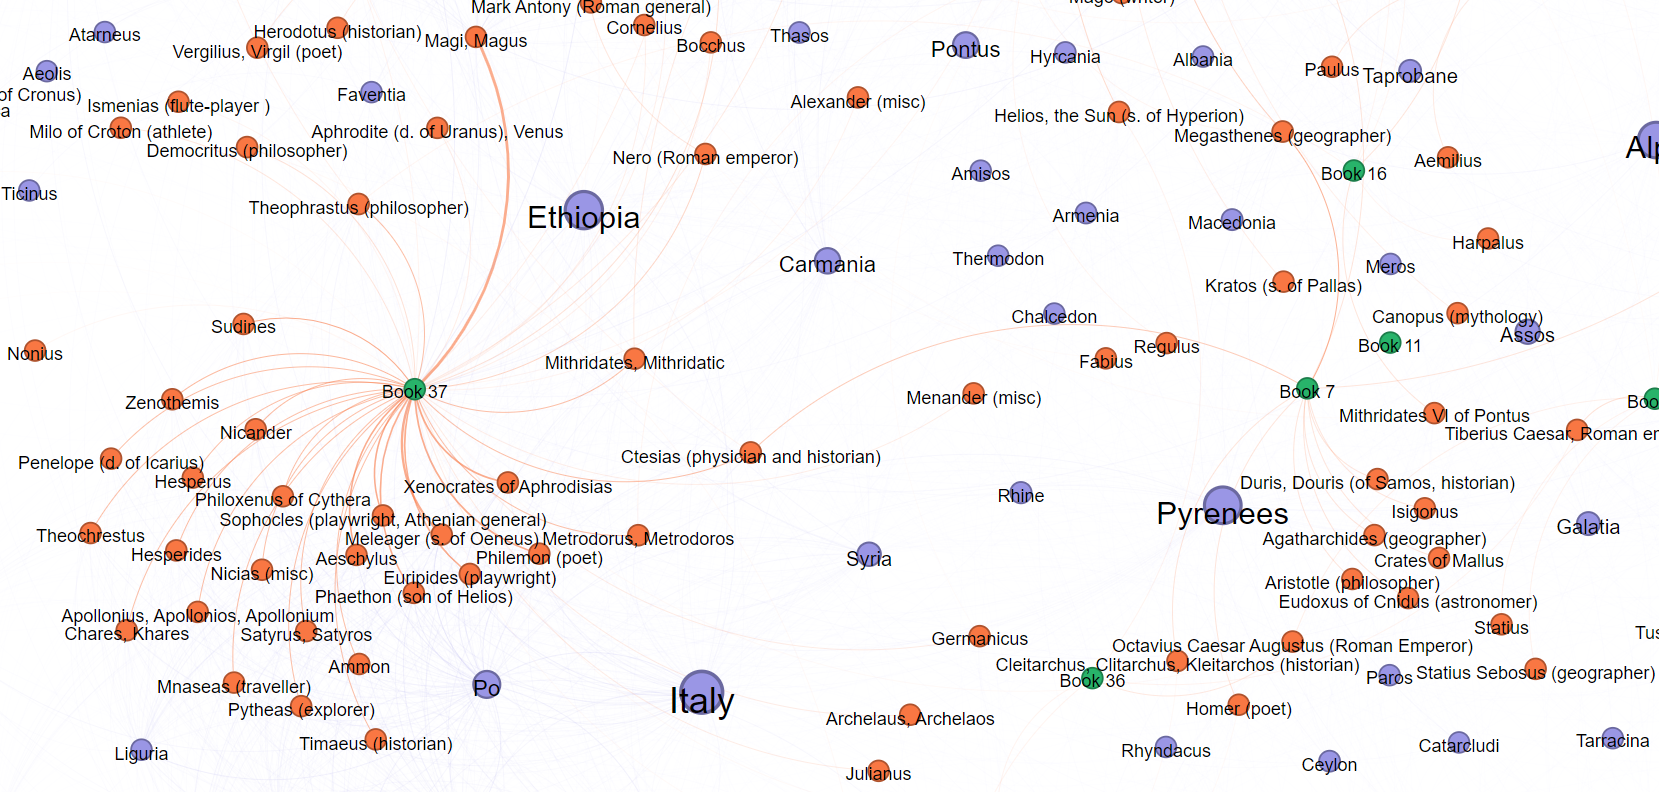
\includegraphics{NHthesis_structure_files/figure-pdf/fig-network_zoom_book37-output-1.png}

}

\caption{\label{fig-network_zoom_book37}Clusters of Book 37 in
India-related content in \emph{Natural History}}

\end{figure}

While in the cluster of Book 37, strong edges are connected to Greek
scholars, such as ``Xenocrates'', ``Aeschylus'', ``Sudines'' and
``Zenothemis''. Also there is a significant connectness with ``Magi'',
referring to the priests in Zoroastrianism, a trditional Persian
religion mentioned in the discussion about tales and myths related to
the precious stones.

An interesting finding in close reading is that in Book 37, Pliny had
addressed direct disprovement to these two groups, with a strong
critical attitude. As quoted in the following paragraphs, the Greek
scholars and Magus are often mentioned as debatable subjects in Book 37,
as a strategy for him to express his own worship of nature and the
material world.

\begin{quote}
37.11.2 ``Here is an opportunity for \textbf{exposing the falsehoods of
the Greeks}.''
\end{quote}

\begin{quote}
37.14.1 ``Now I shall discuss those kinds of gemstones that are
acknowledged as such, beginning with the finest. And this shall not be
my only aim, but to the greater profit of mankind \textbf{I shall
incidentally confute the abominable falsehoods of the Magi}, since in
very many of their statements about gems they have gone far beyond
providing an alluring substitute for medical science into the realms of
the supernatural.''
\end{quote}

To sum up, the network graph visualizes the connectedness between
different types of clustered entities and the central entities within
the narrative. In this study, taking the relationship of the place
names, person names and book numbers in the target text into
consideration, it shows clearly that India is the center of the
narrative, and Arabia and Egypt are closely connected to this center.
Also, it depicted how the person names of history figures, mythological
gods, explorers and scholars are located in the narrative, shedding a
light on the structure of the India-related content in \emph{Natural
History}.

If including more types of entities, such as animals, events, ethnic
groups, into the network, it will contribute to a more nuanced distance
map and entity clustering, which shows more dimensions of the content
structure.

\hypertarget{sec-conclusions}{%
\section{Conclusions}\label{sec-conclusions}}

\hypertarget{comprehension-of-india-in-the-narrative}{%
\subsection{Comprehension of ``India'' in the
narrative}\label{comprehension-of-india-in-the-narrative}}

Leading by the research questions of ``How is India described, and how
is the information about India structured in the work?'', the above
analysis of different methods, including word frequency and collocation
pattern observation, topic modeling and network analysis, integrating
with close reading of the text, comprise a comprehension of ``India'' in
the narrative of \emph{Natural History}.

Generally, India is regarded as a significant geographical contrast to
the Roman Empire and the Mediterranean. It is frequently mentioned for
comparison in the description of landscape, expedition, navigating or
trading routes and origins of natural creatures and elements of other
locations. And the name of rivers in Indian subcontinent, including some
tributaries, are given a highlight as references. Another important role
of India in the narrative is a major trading partner who frequently
import rare and precious treasures into the Mediterranean.

More specifically, the content about India is potentially themed in
three topics, integrating with a close reading of the text, these three
topics can be illustrated in details. The more prominent topics are the
geographical and social condition aobut Indian nations and stones
originated and produced in India. In the former topic, inspite of
addressing India as a origin for numerous marvels, Pliny incidentally
mentioned the epic tales or history related to the conquest of India,
which suggest an imperial perspective of the work. And in the less
prominent topic, which focused on the merchandise trade, Pliny expressed
his criticism about the human greed and unnecessary interference on
nature it reflects, which echos his Stoic claim of nature and human
world.

And a network of place names, person names and book numbers of the
India-related text has been created to depict the focus and co-occurence
clusters in the content structure. It shows that Arabia and Ethopia are
the two places that close to the mentioning of India in the text, and
for different books, there are specific history figures and referencing
scholars clustering aroud. And an interesting observation is that in the
person name cluster of Book 37, which discussed about the gemstones,
Mangus and Geek scholars played an important role as disproving
subjects, for Pliny to express his advocate worshiping the genuine
nature and material world as a Stoic.

In summary, in Pliny's unintentional portrait, India showed its
complexity as a geographical contrast, an origin of marvels and
treasures, a major trading partner, and a context of unecessary
luxurious pursuit of Pliny's contemporary that he debate against in the
scope of \emph{Natural History}.

\hypertarget{distant-reading-as-a-method}{%
\subsection{Distant reading as a
method}\label{distant-reading-as-a-method}}

The attempt of utilizing several distant reading methods for a research
of classical text in this study has, to a certain extent, achieved a
response to the research question.

From pinning down the research question to conducting a meticulous
analysis of the designated text, the application of distant reading
methods yielded insightful perspectives and enriched information.
However, as shown in the topic modeling section of Data analysis, an
integration of close reading is essential in interpreting the outputs of
distant reading.

Furthermore, when implementing these methods, data completeness check
and validation are crucial steps to be taken before running the
analysis. Since the sophisticated textual contents are simplified and
restructured as data values in tablular format, it will make big
difference for the outcome of missing or mistaken inputs.

Another benefit of adopting the distant reading approaches is the output
dataset can be repurposed for subsequent investigations. Together with
this thesis, the following dataset and outputs are available on the
\href{https://github.com/lizaodawn/NH_thesis}{GitHub repository} for
potentially re-uses:

\begin{enumerate}
\def\labelenumi{\arabic{enumi}.}
\tightlist
\item
  Dataset of Indian place names mentioned in \emph{Natural Hisoty} with
  the coordinating textual passages (scraped from TOPOSText with
  supplemented mannually checked annotations)
\item
  Dataset of geographical names menttioned in \emph{Natural History}
  with the coordinating textual passages (scraped from TOPOSText)
\item
  Corpus files of textual passages from the \emph{Natural History}
  related to India
\item
  Network graph of place names, person names and book numbers about
  India-related contents in \emph{Natural History}
\end{enumerate}

Beyond that, the presentation of this thesis is practiced in an
integration of \href{https://quarto.org/}{Quarto} with jupyter notebook.
Embedding the YAML metadata into the notebook, it helped mekke a decent
presentation both in HTML and PDF format. With rendering the output in
HTML, the interactive maps and graphs can be published online.

\hypertarget{reflection-and-limitation}{%
\subsection{Reflection and limitation}\label{reflection-and-limitation}}

Though making the best effort to conduct a complete and consistent study
for this thesis, there are still some limitation in the data
preprocessing and parameter tuning sections that could be enhanced.

As introduced in the Data preparation section, the Indian place names
scraped from TOPOSText is found incomplete and gone through a mannual
check. About 24\% of the amount of orignal retrieved dataset were
appended after the mannual check. Though the supplemented Indian place
annotation has been updated to the dataset compelling all geographical
annotations, there might be missing identifications of places outside
the specified coordinates range for India, which is better to also go
through a mannual check and suppliment. However, as it requires more
effort and time for the scale of the current study, the step has not
been taken. It will make the dataset more complete and the context for
this study more consistent if the same supplimenting process of all
place names could be done.

And for the topic modelling section, when deciding the topic numer and
passed for assigning the topics, though there is a validation process
for topic number designation, and it aligns with the intuitive
observation about differnt outputs, it is better to go through
validation other parameters and general comparison for a more validating
fine tuning.

On the other hand, with time limitation, it only added person name as an
additional entity node for the network analysis. The current network
graph shows the distance relationship between person names, place names
and book numbers. It may give more dimensions for the whole content
structure when including more types of entities, as animals, events, and
ethnic groups, which are available on the TOPOSText annotations. In this
regard, if the study will continues in the future, this aspect can be
certainlly enhanced.

And for the presentation of network graph, alternative platforms should
be explored for a more interactive output. The optimal scheme is to make
the graph easily zooming in to different clusters, and filtering with
different types of nodes.

\newpage

\hypertarget{references}{%
\section*{References}\label{references}}
\addcontentsline{toc}{section}{References}

\hypertarget{refs}{}
\begin{CSLReferences}{1}{0}
\leavevmode\vadjust pre{\hypertarget{ref-akbik2018coling}{}}%
Akbik, Alan, Duncan Blythe, and Roland Vollgraf. 2018. {``Contextual
String Embeddings for Sequence Labeling.''} In \emph{{COLING} 2018, 27th
International Conference on Computational Linguistics}, 1638--49.

\leavevmode\vadjust pre{\hypertarget{ref-bail}{}}%
Bail, Christopher A. n.d. {``Topic {Modeling}.''} Accessed August 3,
2023.
\url{https://cbail.github.io/textasdata/topic-modeling/rmarkdown/Topic_Modeling.html}.

\leavevmode\vadjust pre{\hypertarget{ref-barber}{}}%
Barber, Jordan. n.d. {``Latent {Dirichlet} {Allocation} ({LDA}) with
{Python}.''} Accessed March 15, 2023.
\url{https://rstudio-pubs-static.s3.amazonaws.com/79360_850b2a69980c4488b1db95987a24867a.html}.

\leavevmode\vadjust pre{\hypertarget{ref-beagon1996}{}}%
Beagon, Mary. 1996. {``Nature and Views of Her Landscapes in {Pliny} the
{Elder}.''} In \emph{Human {Landscapes} in {Classical} {Antiquity}},
285--309. Routledge.

\leavevmode\vadjust pre{\hypertarget{ref-beagon2011}{}}%
---------. 2011. {``Chapter {Five}. {The} {Curious} {Eye} {Of} {The}
{Elder} {Pliny}.''} In \emph{Pliny the {Elder}: {Themes} and
{Contexts}}, 71--88. Brill.
\url{https://brill.com/display/book/edcoll/9789004210073/Bej.9789004202344.i-248_006.xml}.

\leavevmode\vadjust pre{\hypertarget{ref-fantoli2022}{}}%
Fantoli, Margherita. 2022. {``Statistics and Linguistics: Can We Tell
Something More about {Pliny} the {Elder}?''}
\url{https://classics-at.chs.harvard.edu/statistics-and-linguistics-can-we-tell-something-more-about-pliny-the-elder/}.

\leavevmode\vadjust pre{\hypertarget{ref-healy1999}{}}%
Healy, John F. 1999. \emph{Pliny the {Elder} on Science and Technology}.
Oxford: university press.

\leavevmode\vadjust pre{\hypertarget{ref-kapadia2022}{}}%
Kapadia, Shashank. 2022. {``Topic {Modeling} in {Python}: {Latent}
{Dirichlet} {Allocation} ({LDA}).''} \emph{Medium}.
\url{https://towardsdatascience.com/end-to-end-topic-modeling-in-python-latent-dirichlet-allocation-lda-35ce4ed6b3e0}.

\leavevmode\vadjust pre{\hypertarget{ref-lao2016}{}}%
Lao, Eugenia. 2016. {``Taxonomic {Organization} in {Pliny}'s {Natural}
{History}.''} In \emph{Greek and {Roman} Poetry, the {Elder} {Pliny}},
edited by Francis Cairns and Roy Gibson, 209--46. Papers of the
{Langford} {Latin} {Seminar} 16. Prenton: Francis Cairns Publications.

\leavevmode\vadjust pre{\hypertarget{ref-murphy2003}{}}%
Murphy, Trevor. 2003. {``11. Pliny{'}s Naturalis Historia: The Prodigal
Text.''} In, 301--22. BRILL.
\url{https://doi.org/10.1163/9789004217157_012}.

\leavevmode\vadjust pre{\hypertarget{ref-naas2002}{}}%
Naas, Valérie. 2002. \emph{Le Projet Encyclopédique de {Pline}
l'{Ancien}}. Collection de l'école Française de {Rome} 303. Rome: Ecole
française de Rome.

\leavevmode\vadjust pre{\hypertarget{ref-naas2011}{}}%
---------. 2011. {``Chapter {Four}. {Imperialism}, {Mirabilia}, {And}
{Knowledge}: {Some} {Paradoxes} {In} {The} {Naturalis} {Historia}.''} In
\emph{Pliny the {Elder}: {Themes} and {Contexts}}, 57--70. Brill.
\url{https://brill.com/display/book/edcoll/9789004210073/Bej.9789004202344.i-248_005.xml}.

\leavevmode\vadjust pre{\hypertarget{ref-neelis2011}{}}%
Neelis, J. 2011. {``Chapter {Three}. {Trade} {Networks} {In} {Ancient}
{South} {Asia}.''} In \emph{Early {Buddhist} {Transmission} and {Trade}
{Networks}}, 183--228. Brill.
\url{https://brill.com/display/book/9789004194588/Bej.9789004181595.i-372_004.xml}.

\leavevmode\vadjust pre{\hypertarget{ref-pinkster2005}{}}%
Pinkster, Harm. 2005. {``The {Language} of {Pliny} the {Elder}.''}
\emph{Journal of Asthma - J ASTHMA} 129 (November): 239--56.
\url{https://doi.org/10.5871/bacad/9780197263327.003.0011}.

\leavevmode\vadjust pre{\hypertarget{ref-pollard2009}{}}%
Pollard, Elizabeth Ann. 2009. {``Pliny's {Natural} {History} and the
{Flavian} {Templum} {Pacis}: {Botanical} {Imperialism} in
{First}-{Century} {C}. {E}. {Rome}.''} \emph{Journal of World History}
20 (3): 309--38. \url{https://www.jstor.org/stable/40542802}.

\leavevmode\vadjust pre{\hypertarget{ref-roller2022}{}}%
Roller, D. W. 2022. {``Introduction.''} In \emph{A {Guide} to the
{Geography} of {Pliny} the {Elder}}, 1--14. Cambridge: Cambridge
University Press. \url{https://doi.org/10.1017/9781108693660.003}.

\leavevmode\vadjust pre{\hypertarget{ref-rydberg-cox2021}{}}%
Rydberg-Cox, Jeff. 2021. {``Modeling the {Sources} and {Topics} of
{Pliny}'s {Natural} {History}.''} \emph{Umanistica Digitale}, no. 11:
217--29. \url{https://doi.org/10.6092/issn.2532-8816/12521}.

\leavevmode\vadjust pre{\hypertarget{ref-schultze2011}{}}%
Schultze, Clemence. 2011. {``Chapter {Ten}. {Encyclopaedic}
{Exemplarity} {In} {Pliny} {The} {Elder}.''} In \emph{Pliny the {Elder}:
{Themes} and {Contexts}}, 167--86. Brill.
\url{https://brill.com/display/book/edcoll/9789004210073/Bej.9789004202344.i-248_011.xml}.

\leavevmode\vadjust pre{\hypertarget{ref-szekely2006}{}}%
Székely, Melinda. 2006. {``Eastern {Trade} of the {Roman} {Empire} Based
on {Pliny} the {Elder}'s {Natural} {History}.''} \emph{Chronica} 6
(January): 199--206.
\url{https://www.proquest.com/docview/2379648941/citation/93A42D142D614235PQ/1}.

\leavevmode\vadjust pre{\hypertarget{ref-talbert2000-1}{}}%
Talbert, Richard J. A. 2000a. \emph{Barrington Atlas of the {Greek} and
{Roman} World: Map-by-Map Directory}. Princeton (N.J.): Princeton
university press.

\leavevmode\vadjust pre{\hypertarget{ref-talbert2000}{}}%
---------. 2000b. \emph{Barrington Atlas of the {Greek} and {Roman}
World.} Princeton (N.J.): Princeton university press.

\leavevmode\vadjust pre{\hypertarget{ref-tedeschi2021}{}}%
Tedeschi, Simone, Valentino Maiorca, Niccolò Campolungo, Francesco
Cecconi, and Roberto Navigli. 2021. {``WikiNEuRal: Combined Neural and
Knowledge-Based Silver Data Creation for Multilingual NER.''} In,
25212533. Punta Cana, Dominican Republic: Association for Computational
Linguistics. \url{https://aclanthology.org/2021.findings-emnlp.215}.

\leavevmode\vadjust pre{\hypertarget{ref-tran2022}{}}%
Tran, Khuyen. 2022. {``pyLDAvis: Topic Modelling Exploration Tool That
Every NLP Data Scientist Should Know.''}
\url{https://neptune.ai/blog/pyldavis-topic-modelling-exploration-tool-that-every-nlp-data-scientist-should-know}.

\leavevmode\vadjust pre{\hypertarget{ref-underwood2012}{}}%
Underwood, Ted. 2012. {``Topic Modeling Made Just Simple Enough.''}
\emph{The Stone and the Shell}.
\url{https://tedunderwood.com/2012/04/07/topic-modeling-made-just-simple-enough/}.

\end{CSLReferences}



\end{document}
